\documentclass[pdflatex,sn-nature]{sn-jnl}

\usepackage{graphicx}
\usepackage{amsmath,amssymb}
\usepackage{booktabs}
\usepackage{xcolor}
\usepackage[T1]{fontenc}
\usepackage{lmodern}
\usepackage{textcomp}
\usepackage{lineno}

\raggedbottom
\setcitestyle{super,open={},close={},comma,sort&compress}
\graphicspath{{../results/figures/v2/}}
% Generated by scripts/make_numbers_tex.py from results/ -- do not edit by hand.
\makeatletter
\newcommand{\val}[1]{\ifcsname val@#1\endcsname\csname val@#1\endcsname\else\textcolor{red}{\textbf{??#1}}\fi}
\expandafter\def\csname val@C:gainret1\endcsname{0.81}
\expandafter\def\csname val@C:gainret120\endcsname{0.33}
\expandafter\def\csname val@C:gainret30\endcsname{0.51}
\expandafter\def\csname val@C:gainret480\endcsname{0.10}
\expandafter\def\csname val@C:gainret7\endcsname{0.72}
\expandafter\def\csname val@C:gainretmax\endcsname{0.81}
\expandafter\def\csname val@C:gainretmin\endcsname{0.10}
\expandafter\def\csname val@C:linown\endcsname{0.26}
\expandafter\def\csname val@C:nnown\endcsname{0.64}
\expandafter\def\csname val@C:nnowndiff\endcsname{0.33}
\expandafter\def\csname val@C:nnowndiffci\endcsname{0.23--0.37}
\expandafter\def\csname val@C:nnpairs\endcsname{55}
\expandafter\def\csname val@C:nnrecmax\endcsname{68}
\expandafter\def\csname val@C:nnrecmin\endcsname{46}
\expandafter\def\csname val@C:nnretdiff\endcsname{0.08}
\expandafter\def\csname val@C:nnretp\endcsname{0.055}
\expandafter\def\csname val@C:ntrain\endcsname{64}
\expandafter\def\csname val@C:pairs\endcsname{145}
\expandafter\def\csname val@C:rec1\endcsname{38}
\expandafter\def\csname val@C:rec120\endcsname{42}
\expandafter\def\csname val@C:rec30\endcsname{28}
\expandafter\def\csname val@C:rec480\endcsname{29}
\expandafter\def\csname val@C:rec7\endcsname{37}
\expandafter\def\csname val@C:recmax\endcsname{42}
\expandafter\def\csname val@C:recmin\endcsname{28}
\expandafter\def\csname val@C:ret1\endcsname{0.71}
\expandafter\def\csname val@C:ret120\endcsname{$-$0.09}
\expandafter\def\csname val@C:ret1ci\endcsname{0.63--0.77}
\expandafter\def\csname val@C:ret30\endcsname{0.25}
\expandafter\def\csname val@C:ret480\endcsname{$-$0.27}
\expandafter\def\csname val@C:ret7\endcsname{0.56}
\expandafter\def\csname val@C:rulealpha\endcsname{10^{4}}
\expandafter\def\csname val@C:rulemax\endcsname{0.032}
\expandafter\def\csname val@C:rulemed\endcsname{0.017}
\expandafter\def\csname val@C:rulemin\endcsname{0.001}
\expandafter\def\csname val@C:rulen\endcsname{40}
\expandafter\def\csname val@C:rulep\endcsname{7.8\times10^{-11}}
\expandafter\def\csname val@C:rulepos\endcsname{39}
\expandafter\def\csname val@C:rulesame\endcsname{0.002}
\expandafter\def\csname val@C:rulevsbest\endcsname{0.000}
\expandafter\def\csname val@C:rulevsbestp\endcsname{0.69}
\expandafter\def\csname val@C:strict1\endcsname{0.70}
\expandafter\def\csname val@C:strict1ci\endcsname{0.58--0.77}
\expandafter\def\csname val@C:strict1n\endcsname{31}
\expandafter\def\csname val@C:strict2\endcsname{0.72}
\expandafter\def\csname val@C:strict2ci\endcsname{0.59--0.92}
\expandafter\def\csname val@C:strict2n\endcsname{11}
\expandafter\def\csname val@C:thalf\endcsname{9.2}
\expandafter\def\csname val@C:thalftuned\endcsname{10}
\expandafter\def\csname val@C:tret1\endcsname{0.73}
\expandafter\def\csname val@C:tret120\endcsname{0.04}
\expandafter\def\csname val@C:tret30\endcsname{0.23}
\expandafter\def\csname val@C:tret480\endcsname{$-$0.17}
\expandafter\def\csname val@C:tret7\endcsname{0.60}
\expandafter\def\csname val@C:tunedabsdiff\endcsname{0.015}
\expandafter\def\csname val@C:tunedabsp\endcsname{3.4\times10^{-11}}
\expandafter\def\csname val@C:tunedfrac\endcsname{94}
\expandafter\def\csname val@C:tunedretdiff\endcsname{0.05}
\expandafter\def\csname val@C:tunedretp\endcsname{8.2\times10^{-12}}
\expandafter\def\csname val@M:coraldiff\endcsname{$-$0.000}
\expandafter\def\csname val@M:coralfrac\endcsname{50}
\expandafter\def\csname val@M:coraln\endcsname{22}
\expandafter\def\csname val@M:coralp\endcsname{0.61}
\expandafter\def\csname val@M:gainret1\endcsname{0.84}
\expandafter\def\csname val@M:gainret120\endcsname{0.35}
\expandafter\def\csname val@M:gainret30\endcsname{0.69}
\expandafter\def\csname val@M:gainret480\endcsname{0.20}
\expandafter\def\csname val@M:gainret7\endcsname{0.70}
\expandafter\def\csname val@M:gainretmax\endcsname{0.84}
\expandafter\def\csname val@M:gainretmin\endcsname{0.20}
\expandafter\def\csname val@M:linown\endcsname{0.30}
\expandafter\def\csname val@M:nnown\endcsname{0.72}
\expandafter\def\csname val@M:nnowndiff\endcsname{0.42}
\expandafter\def\csname val@M:nnowndiffci\endcsname{0.34--0.47}
\expandafter\def\csname val@M:nnpairs\endcsname{44}
\expandafter\def\csname val@M:nnrecmax\endcsname{69}
\expandafter\def\csname val@M:nnrecmin\endcsname{48}
\expandafter\def\csname val@M:nnretdiff\endcsname{$-$0.15}
\expandafter\def\csname val@M:nnretp\endcsname{2.1\times10^{-4}}
\expandafter\def\csname val@M:ntrain\endcsname{22}
\expandafter\def\csname val@M:pairs\endcsname{44}
\expandafter\def\csname val@M:rec1\endcsname{24}
\expandafter\def\csname val@M:rec120\endcsname{35}
\expandafter\def\csname val@M:rec30\endcsname{32}
\expandafter\def\csname val@M:rec480\endcsname{19}
\expandafter\def\csname val@M:rec7\endcsname{26}
\expandafter\def\csname val@M:recmax\endcsname{35}
\expandafter\def\csname val@M:recmin\endcsname{19}
\expandafter\def\csname val@M:ret1\endcsname{0.77}
\expandafter\def\csname val@M:ret120\endcsname{0.04}
\expandafter\def\csname val@M:ret1ci\endcsname{0.71--0.84}
\expandafter\def\csname val@M:ret30\endcsname{0.55}
\expandafter\def\csname val@M:ret480\endcsname{0.02}
\expandafter\def\csname val@M:ret7\endcsname{0.60}
\expandafter\def\csname val@M:rulealpha\endcsname{10^{3}}
\expandafter\def\csname val@M:rulemax\endcsname{0.001}
\expandafter\def\csname val@M:rulemed\endcsname{0.001}
\expandafter\def\csname val@M:rulemin\endcsname{0.000}
\expandafter\def\csname val@M:rulen\endcsname{22}
\expandafter\def\csname val@M:rulep\endcsname{2.1\times10^{-4}}
\expandafter\def\csname val@M:rulepos\endcsname{19}
\expandafter\def\csname val@M:rulesame\endcsname{0.000}
\expandafter\def\csname val@M:rulevsbest\endcsname{0.000}
\expandafter\def\csname val@M:rulevsbestp\endcsname{0.16}
\expandafter\def\csname val@M:stabfixdiff\endcsname{$-$0.090}
\expandafter\def\csname val@M:stabfixfrac\endcsname{0}
\expandafter\def\csname val@M:stabfixn\endcsname{22}
\expandafter\def\csname val@M:stabfixp\endcsname{4.8\times10^{-7}}
\expandafter\def\csname val@M:stabrendiff\endcsname{$-$0.136}
\expandafter\def\csname val@M:stabrenfrac\endcsname{5}
\expandafter\def\csname val@M:stabrenn\endcsname{22}
\expandafter\def\csname val@M:stabrenp\endcsname{4.8\times10^{-6}}
\expandafter\def\csname val@M:strict1\endcsname{0.80}
\expandafter\def\csname val@M:strict1ci\endcsname{0.70--0.86}
\expandafter\def\csname val@M:strict1n\endcsname{12}
\expandafter\def\csname val@M:strict2n\endcsname{2}
\expandafter\def\csname val@M:thalf\endcsname{34}
\expandafter\def\csname val@M:thalftuned\endcsname{37}
\expandafter\def\csname val@M:tret1\endcsname{0.81}
\expandafter\def\csname val@M:tret120\endcsname{0.09}
\expandafter\def\csname val@M:tret30\endcsname{0.57}
\expandafter\def\csname val@M:tret480\endcsname{0.04}
\expandafter\def\csname val@M:tret7\endcsname{0.62}
\expandafter\def\csname val@M:tunedabsdiff\endcsname{0.005}
\expandafter\def\csname val@M:tunedabsp\endcsname{0.007}
\expandafter\def\csname val@M:tunedfrac\endcsname{82}
\expandafter\def\csname val@M:tunedretdiff\endcsname{0.01}
\expandafter\def\csname val@M:tunedretp\endcsname{0.017}
\expandafter\def\csname val@N:coraldiff\endcsname{0.011}
\expandafter\def\csname val@N:coralfrac\endcsname{79}
\expandafter\def\csname val@N:coraln\endcsname{80}
\expandafter\def\csname val@N:coralp\endcsname{1.9\times10^{-9}}
\expandafter\def\csname val@N:gainret1\endcsname{0.78}
\expandafter\def\csname val@N:gainret120\endcsname{0.34}
\expandafter\def\csname val@N:gainret30\endcsname{0.43}
\expandafter\def\csname val@N:gainret480\endcsname{0.22}
\expandafter\def\csname val@N:gainret7\endcsname{0.63}
\expandafter\def\csname val@N:gainretmax\endcsname{0.78}
\expandafter\def\csname val@N:gainretmin\endcsname{0.22}
\expandafter\def\csname val@N:linown\endcsname{0.28}
\expandafter\def\csname val@N:nnown\endcsname{0.39}
\expandafter\def\csname val@N:nnowndiff\endcsname{0.11}
\expandafter\def\csname val@N:nnowndiffci\endcsname{0.10--0.12}
\expandafter\def\csname val@N:nnpairs\endcsname{81}
\expandafter\def\csname val@N:nnrecmax\endcsname{63}
\expandafter\def\csname val@N:nnrecmin\endcsname{36}
\expandafter\def\csname val@N:nnretdiff\endcsname{0.23}
\expandafter\def\csname val@N:nnretp\endcsname{1.2\times10^{-7}}
\expandafter\def\csname val@N:ntrain\endcsname{80}
\expandafter\def\csname val@N:pairs\endcsname{259}
\expandafter\def\csname val@N:rec1\endcsname{26}
\expandafter\def\csname val@N:rec120\endcsname{30}
\expandafter\def\csname val@N:rec30\endcsname{27}
\expandafter\def\csname val@N:rec480\endcsname{34}
\expandafter\def\csname val@N:rec7\endcsname{14}
\expandafter\def\csname val@N:recmax\endcsname{34}
\expandafter\def\csname val@N:recmin\endcsname{14}
\expandafter\def\csname val@N:renmeandiff\endcsname{0.061}
\expandafter\def\csname val@N:renmeanfrac\endcsname{85}
\expandafter\def\csname val@N:renmeann\endcsname{79}
\expandafter\def\csname val@N:renmeanp\endcsname{3.0\times10^{-11}}
\expandafter\def\csname val@N:ret1\endcsname{0.73}
\expandafter\def\csname val@N:ret120\endcsname{0.04}
\expandafter\def\csname val@N:ret1ci\endcsname{0.62--0.78}
\expandafter\def\csname val@N:ret30\endcsname{0.19}
\expandafter\def\csname val@N:ret480\endcsname{$-$0.36}
\expandafter\def\csname val@N:ret7\endcsname{0.54}
\expandafter\def\csname val@N:rotmeandiff\endcsname{$-$0.063}
\expandafter\def\csname val@N:rotmeanfrac\endcsname{18}
\expandafter\def\csname val@N:rotmeann\endcsname{79}
\expandafter\def\csname val@N:rotmeanp\endcsname{3.4\times10^{-8}}
\expandafter\def\csname val@N:rotrendiff\endcsname{$-$0.019}
\expandafter\def\csname val@N:rotrenfrac\endcsname{19}
\expandafter\def\csname val@N:rotrenn\endcsname{79}
\expandafter\def\csname val@N:rotrenp\endcsname{6.6\times10^{-9}}
\expandafter\def\csname val@N:rulealpha\endcsname{10^{4}}
\expandafter\def\csname val@N:rulemax\endcsname{0.090}
\expandafter\def\csname val@N:rulemed\endcsname{0.060}
\expandafter\def\csname val@N:rulemin\endcsname{0.021}
\expandafter\def\csname val@N:rulen\endcsname{40}
\expandafter\def\csname val@N:rulep\endcsname{1.8\times10^{-12}}
\expandafter\def\csname val@N:rulepos\endcsname{40}
\expandafter\def\csname val@N:rulesame\endcsname{0.003}
\expandafter\def\csname val@N:rulevsbest\endcsname{0.004}
\expandafter\def\csname val@N:rulevsbestp\endcsname{6.9\times10^{-5}}
\expandafter\def\csname val@N:stabfixdiff\endcsname{$-$0.008}
\expandafter\def\csname val@N:stabfixfrac\endcsname{36}
\expandafter\def\csname val@N:stabfixn\endcsname{80}
\expandafter\def\csname val@N:stabfixp\endcsname{0.015}
\expandafter\def\csname val@N:stabrendiff\endcsname{$-$0.018}
\expandafter\def\csname val@N:stabrenfrac\endcsname{42}
\expandafter\def\csname val@N:stabrenn\endcsname{80}
\expandafter\def\csname val@N:stabrenp\endcsname{0.55}
\expandafter\def\csname val@N:strict1\endcsname{0.74}
\expandafter\def\csname val@N:strict1ci\endcsname{0.62--0.83}
\expandafter\def\csname val@N:strict1n\endcsname{21}
\expandafter\def\csname val@N:strict2\endcsname{0.64}
\expandafter\def\csname val@N:strict2ci\endcsname{0.20--0.80}
\expandafter\def\csname val@N:strict2n\endcsname{9}
\expandafter\def\csname val@N:thalf\endcsname{8.1}
\expandafter\def\csname val@N:thalftuned\endcsname{16}
\expandafter\def\csname val@N:tret1\endcsname{0.79}
\expandafter\def\csname val@N:tret120\endcsname{0.30}
\expandafter\def\csname val@N:tret30\endcsname{0.41}
\expandafter\def\csname val@N:tret480\endcsname{0.01}
\expandafter\def\csname val@N:tret7\endcsname{0.63}
\expandafter\def\csname val@N:tunedabsdiff\endcsname{0.061}
\expandafter\def\csname val@N:tunedabsp\endcsname{8.2\times10^{-15}}
\expandafter\def\csname val@N:tunedfrac\endcsname{99}
\expandafter\def\csname val@N:tunedretdiff\endcsname{0.22}
\expandafter\def\csname val@N:tunedretp\endcsname{8.2\times10^{-15}}
\expandafter\def\csname val@T11:mf:dayr\endcsname{$-$0.09}
\expandafter\def\csname val@T11:mf:days\endcsname{17.1}
\expandafter\def\csname val@T11:mf:dn\endcsname{17.5}
\expandafter\def\csname val@T11:mf:do\endcsname{11.9}
\expandafter\def\csname val@T11:mf:k\endcsname{29.0}
\expandafter\def\csname val@T11:mf:npart\endcsname{0.37}
\expandafter\def\csname val@T11:mf:nraw\endcsname{0.82}
\expandafter\def\csname val@T11:mf:o\endcsname{12.8}
\expandafter\def\csname val@T11:mf:opart\endcsname{0.73}
\expandafter\def\csname val@T11:mf:oraw\endcsname{0.81}
\expandafter\def\csname val@T11:mf:rdays\endcsname{0.84}
\expandafter\def\csname val@T11:mf:win\endcsname{145}
\expandafter\def\csname val@T5:coraldiff\endcsname{$-$0.081}
\expandafter\def\csname val@T5:coralfrac\endcsname{16}
\expandafter\def\csname val@T5:coraln\endcsname{32}
\expandafter\def\csname val@T5:coralp\endcsname{2.8\times10^{-4}}
\expandafter\def\csname val@T5:gainret1\endcsname{0.92}
\expandafter\def\csname val@T5:gainret120\endcsname{0.78}
\expandafter\def\csname val@T5:gainret30\endcsname{0.80}
\expandafter\def\csname val@T5:gainret480\endcsname{0.83}
\expandafter\def\csname val@T5:gainret7\endcsname{0.89}
\expandafter\def\csname val@T5:gainretmax\endcsname{0.92}
\expandafter\def\csname val@T5:gainretmin\endcsname{0.78}
\expandafter\def\csname val@T5:linown\endcsname{0.50}
\expandafter\def\csname val@T5:mf:dayr\endcsname{0.60}
\expandafter\def\csname val@T5:mf:days\endcsname{32.9}
\expandafter\def\csname val@T5:mf:dn\endcsname{38.3}
\expandafter\def\csname val@T5:mf:do\endcsname{20.8}
\expandafter\def\csname val@T5:mf:k\endcsname{19.9}
\expandafter\def\csname val@T5:mf:npart\endcsname{0.49}
\expandafter\def\csname val@T5:mf:nraw\endcsname{0.50}
\expandafter\def\csname val@T5:mf:o\endcsname{15.0}
\expandafter\def\csname val@T5:mf:opart\endcsname{0.78}
\expandafter\def\csname val@T5:mf:oraw\endcsname{0.79}
\expandafter\def\csname val@T5:mf:rdays\endcsname{0.17}
\expandafter\def\csname val@T5:mf:win\endcsname{73}
\expandafter\def\csname val@T5:nnown\endcsname{0.49}
\expandafter\def\csname val@T5:nnowndiff\endcsname{$-$0.03}
\expandafter\def\csname val@T5:nnowndiffci\endcsname{$-$0.04--$-$0.01}
\expandafter\def\csname val@T5:nnpairs\endcsname{71}
\expandafter\def\csname val@T5:nnrecmax\endcsname{92}
\expandafter\def\csname val@T5:nnrecmin\endcsname{82}
\expandafter\def\csname val@T5:nnretdiff\endcsname{$-$0.49}
\expandafter\def\csname val@T5:nnretp\endcsname{0.017}
\expandafter\def\csname val@T5:ntrain\endcsname{89}
\expandafter\def\csname val@T5:pairs\endcsname{256}
\expandafter\def\csname val@T5:rec1\endcsname{76}
\expandafter\def\csname val@T5:rec120\endcsname{78}
\expandafter\def\csname val@T5:rec30\endcsname{72}
\expandafter\def\csname val@T5:rec480\endcsname{85}
\expandafter\def\csname val@T5:rec7\endcsname{78}
\expandafter\def\csname val@T5:recmax\endcsname{85}
\expandafter\def\csname val@T5:recmin\endcsname{72}
\expandafter\def\csname val@T5:ret1\endcsname{0.61}
\expandafter\def\csname val@T5:ret120\endcsname{0.01}
\expandafter\def\csname val@T5:ret1ci\endcsname{0.34--0.76}
\expandafter\def\csname val@T5:ret30\endcsname{0.09}
\expandafter\def\csname val@T5:ret480\endcsname{$-$0.32}
\expandafter\def\csname val@T5:ret7\endcsname{0.44}
\expandafter\def\csname val@T5:rulealpha\endcsname{10^{4}}
\expandafter\def\csname val@T5:rulemax\endcsname{0.040}
\expandafter\def\csname val@T5:rulemed\endcsname{0.033}
\expandafter\def\csname val@T5:rulemin\endcsname{0.018}
\expandafter\def\csname val@T5:rulen\endcsname{40}
\expandafter\def\csname val@T5:rulep\endcsname{1.8\times10^{-12}}
\expandafter\def\csname val@T5:rulepos\endcsname{40}
\expandafter\def\csname val@T5:rulesame\endcsname{0.008}
\expandafter\def\csname val@T5:stabfixdiff\endcsname{0.044}
\expandafter\def\csname val@T5:stabfixfrac\endcsname{75}
\expandafter\def\csname val@T5:stabfixn\endcsname{32}
\expandafter\def\csname val@T5:stabfixp\endcsname{0.062}
\expandafter\def\csname val@T5:stabrendiff\endcsname{0.125}
\expandafter\def\csname val@T5:stabrenfrac\endcsname{78}
\expandafter\def\csname val@T5:stabrenn\endcsname{32}
\expandafter\def\csname val@T5:stabrenp\endcsname{1.3\times10^{-5}}
\expandafter\def\csname val@T5:strict1n\endcsname{2}
\expandafter\def\csname val@T5:strict2\endcsname{0.59}
\expandafter\def\csname val@T5:strict2ci\endcsname{$-$0.07--0.70}
\expandafter\def\csname val@T5:strict2n\endcsname{15}
\expandafter\def\csname val@T5:thalf\endcsname{3.7}
\expandafter\def\csname val@T6:coraldiff\endcsname{$-$0.011}
\expandafter\def\csname val@T6:coralfrac\endcsname{30}
\expandafter\def\csname val@T6:coraln\endcsname{33}
\expandafter\def\csname val@T6:coralp\endcsname{0.23}
\expandafter\def\csname val@T6:gainret1\endcsname{0.90}
\expandafter\def\csname val@T6:gainret120\endcsname{0.84}
\expandafter\def\csname val@T6:gainret30\endcsname{0.94}
\expandafter\def\csname val@T6:gainret480\endcsname{0.81}
\expandafter\def\csname val@T6:gainret7\endcsname{0.96}
\expandafter\def\csname val@T6:gainretmax\endcsname{0.96}
\expandafter\def\csname val@T6:gainretmin\endcsname{0.81}
\expandafter\def\csname val@T6:linown\endcsname{0.25}
\expandafter\def\csname val@T6:nnown\endcsname{0.24}
\expandafter\def\csname val@T6:nnowndiff\endcsname{$-$0.01}
\expandafter\def\csname val@T6:nnowndiffci\endcsname{$-$0.04--0.00}
\expandafter\def\csname val@T6:nnpairs\endcsname{78}
\expandafter\def\csname val@T6:nnrecmax\endcsname{102}
\expandafter\def\csname val@T6:nnrecmin\endcsname{75}
\expandafter\def\csname val@T6:nnretdiff\endcsname{$-$0.21}
\expandafter\def\csname val@T6:nnretp\endcsname{0.080}
\expandafter\def\csname val@T6:ntrain\endcsname{122}
\expandafter\def\csname val@T6:pairs\endcsname{369}
\expandafter\def\csname val@T6:rec1\endcsname{64}
\expandafter\def\csname val@T6:rec120\endcsname{71}
\expandafter\def\csname val@T6:rec30\endcsname{76}
\expandafter\def\csname val@T6:rec480\endcsname{81}
\expandafter\def\csname val@T6:rec7\endcsname{74}
\expandafter\def\csname val@T6:recmax\endcsname{81}
\expandafter\def\csname val@T6:recmin\endcsname{64}
\expandafter\def\csname val@T6:ret1\endcsname{0.73}
\expandafter\def\csname val@T6:ret120\endcsname{0.51}
\expandafter\def\csname val@T6:ret1ci\endcsname{0.41--0.88}
\expandafter\def\csname val@T6:ret30\endcsname{0.71}
\expandafter\def\csname val@T6:ret480\endcsname{0.30}
\expandafter\def\csname val@T6:ret7\endcsname{0.66}
\expandafter\def\csname val@T6:rulealpha\endcsname{10^{4}}
\expandafter\def\csname val@T6:rulemax\endcsname{0.025}
\expandafter\def\csname val@T6:rulemed\endcsname{0.021}
\expandafter\def\csname val@T6:rulemin\endcsname{0.011}
\expandafter\def\csname val@T6:rulen\endcsname{40}
\expandafter\def\csname val@T6:rulep\endcsname{1.8\times10^{-12}}
\expandafter\def\csname val@T6:rulepos\endcsname{40}
\expandafter\def\csname val@T6:rulesame\endcsname{0.008}
\expandafter\def\csname val@T6:rulevsbest\endcsname{0.000}
\expandafter\def\csname val@T6:rulevsbestp\endcsname{0.39}
\expandafter\def\csname val@T6:stabfixdiff\endcsname{$-$0.012}
\expandafter\def\csname val@T6:stabfixfrac\endcsname{27}
\expandafter\def\csname val@T6:stabfixn\endcsname{33}
\expandafter\def\csname val@T6:stabfixp\endcsname{0.29}
\expandafter\def\csname val@T6:stabrendiff\endcsname{$-$0.004}
\expandafter\def\csname val@T6:stabrenfrac\endcsname{48}
\expandafter\def\csname val@T6:stabrenn\endcsname{33}
\expandafter\def\csname val@T6:stabrenp\endcsname{0.30}
\expandafter\def\csname val@T6:strict1\endcsname{0.41}
\expandafter\def\csname val@T6:strict1ci\endcsname{$-$2.45--0.99}
\expandafter\def\csname val@T6:strict1n\endcsname{5}
\expandafter\def\csname val@T6:strict2\endcsname{0.79}
\expandafter\def\csname val@T6:strict2ci\endcsname{0.50--0.92}
\expandafter\def\csname val@T6:strict2n\endcsname{19}
\expandafter\def\csname val@T6:thalf\endcsname{125}
\expandafter\def\csname val@T6:thalftuned\endcsname{229}
\expandafter\def\csname val@T6:tret1\endcsname{0.80}
\expandafter\def\csname val@T6:tret120\endcsname{0.59}
\expandafter\def\csname val@T6:tret30\endcsname{0.72}
\expandafter\def\csname val@T6:tret480\endcsname{0.39}
\expandafter\def\csname val@T6:tret7\endcsname{0.70}
\expandafter\def\csname val@T6:tunedabsdiff\endcsname{0.019}
\expandafter\def\csname val@T6:tunedabsp\endcsname{9.2\times10^{-22}}
\expandafter\def\csname val@T6:tunedfrac\endcsname{100}
\expandafter\def\csname val@T6:tunedretdiff\endcsname{0.03}
\expandafter\def\csname val@T6:tunedretp\endcsname{0.015}
\expandafter\def\csname val@T9:gainret1\endcsname{0.87}
\expandafter\def\csname val@T9:gainret120\endcsname{0.77}
\expandafter\def\csname val@T9:gainret30\endcsname{0.83}
\expandafter\def\csname val@T9:gainret480\endcsname{0.70}
\expandafter\def\csname val@T9:gainret7\endcsname{0.90}
\expandafter\def\csname val@T9:gainretmax\endcsname{0.90}
\expandafter\def\csname val@T9:gainretmin\endcsname{0.70}
\expandafter\def\csname val@T9:linown\endcsname{0.29}
\expandafter\def\csname val@T9:nnown\endcsname{0.20}
\expandafter\def\csname val@T9:nnowndiff\endcsname{$-$0.06}
\expandafter\def\csname val@T9:nnowndiffci\endcsname{$-$0.09--$-$0.02}
\expandafter\def\csname val@T9:nnpairs\endcsname{50}
\expandafter\def\csname val@T9:nnrecmax\endcsname{121}
\expandafter\def\csname val@T9:nnrecmin\endcsname{75}
\expandafter\def\csname val@T9:nnretdiff\endcsname{0.30}
\expandafter\def\csname val@T9:nnretp\endcsname{0.30}
\expandafter\def\csname val@T9:ntrain\endcsname{114}
\expandafter\def\csname val@T9:pairs\endcsname{361}
\expandafter\def\csname val@T9:rec1\endcsname{76}
\expandafter\def\csname val@T9:rec120\endcsname{82}
\expandafter\def\csname val@T9:rec30\endcsname{78}
\expandafter\def\csname val@T9:rec480\endcsname{81}
\expandafter\def\csname val@T9:rec7\endcsname{84}
\expandafter\def\csname val@T9:recmax\endcsname{84}
\expandafter\def\csname val@T9:recmin\endcsname{76}
\expandafter\def\csname val@T9:ret1\endcsname{0.51}
\expandafter\def\csname val@T9:ret120\endcsname{0.10}
\expandafter\def\csname val@T9:ret1ci\endcsname{0.32--0.66}
\expandafter\def\csname val@T9:ret30\endcsname{0.24}
\expandafter\def\csname val@T9:ret480\endcsname{$-$0.47}
\expandafter\def\csname val@T9:ret7\endcsname{0.39}
\expandafter\def\csname val@T9:rulealpha\endcsname{3\times10^{4}}
\expandafter\def\csname val@T9:rulemax\endcsname{0.043}
\expandafter\def\csname val@T9:rulemed\endcsname{0.045}
\expandafter\def\csname val@T9:rulemin\endcsname{0.029}
\expandafter\def\csname val@T9:rulen\endcsname{40}
\expandafter\def\csname val@T9:rulep\endcsname{1.8\times10^{-12}}
\expandafter\def\csname val@T9:rulepos\endcsname{40}
\expandafter\def\csname val@T9:rulesame\endcsname{0.007}
\expandafter\def\csname val@T9:strict1\endcsname{0.58}
\expandafter\def\csname val@T9:strict1ci\endcsname{0.33--0.76}
\expandafter\def\csname val@T9:strict1n\endcsname{19}
\expandafter\def\csname val@T9:strict2\endcsname{0.34}
\expandafter\def\csname val@T9:strict2ci\endcsname{$-$2.77--0.63}
\expandafter\def\csname val@T9:strict2n\endcsname{8}
\expandafter\def\csname val@T9:thalf\endcsname{1.1}
\expandafter\def\csname val@aug:multi\endcsname{0.056}
\expandafter\def\csname val@aug:pert\endcsname{0.000}
\expandafter\def\csname val@aug:ridge_reg\endcsname{0.042}
\expandafter\def\csname val@aug:sim\endcsname{0.010}
\expandafter\def\csname val@aug:sim_reg\endcsname{0.015}
\expandafter\def\csname val@edge:adj:med\endcsname{$-$0.08}
\expandafter\def\csname val@edge:adj:n\endcsname{17}
\expandafter\def\csname val@edge:adj:neg\endcsname{12}
\expandafter\def\csname val@edge:adj:sign\endcsname{0.072}
\expandafter\def\csname val@edge:adj:wil\endcsname{0.087}
\expandafter\def\csname val@edge:dist:med\endcsname{$-$0.15}
\expandafter\def\csname val@edge:dist:n\endcsname{17}
\expandafter\def\csname val@edge:dist:neg\endcsname{13}
\expandafter\def\csname val@edge:dist:sign\endcsname{0.025}
\expandafter\def\csname val@edge:dist:wil\endcsname{0.013}
\expandafter\def\csname val@edge:raw:med\endcsname{$-$0.11}
\expandafter\def\csname val@edge:raw:n\endcsname{17}
\expandafter\def\csname val@edge:raw:neg\endcsname{13}
\expandafter\def\csname val@edge:raw:sign\endcsname{0.025}
\expandafter\def\csname val@edge:raw:wil\endcsname{0.036}
\expandafter\def\csname val@harm:100:cv\endcsname{0.0}
\expandafter\def\csname val@harm:100:hist\endcsname{1.2}
\expandafter\def\csname val@harm:10:cv\endcsname{10.5}
\expandafter\def\csname val@harm:10:hist\endcsname{1.2}
\expandafter\def\csname val@harm:20:cv\endcsname{8.1}
\expandafter\def\csname val@harm:20:hist\endcsname{0.0}
\expandafter\def\csname val@harm:300:cv\endcsname{0.0}
\expandafter\def\csname val@harm:300:hist\endcsname{0.0}
\expandafter\def\csname val@harm:50:cv\endcsname{1.2}
\expandafter\def\csname val@harm:50:hist\endcsname{0.0}
\expandafter\def\csname val@kw:H\endcsname{11.4}
\expandafter\def\csname val@kw:P\endcsname{0.045}
\expandafter\def\csname val@kw:df\endcsname{5}
\expandafter\def\csname val@mcn:100:cv\endcsname{0}
\expandafter\def\csname val@mcn:100:holm\endcsname{1.00}
\expandafter\def\csname val@mcn:100:p\endcsname{1.00}
\expandafter\def\csname val@mcn:10:cv\endcsname{8}
\expandafter\def\csname val@mcn:10:holm\endcsname{0.039}
\expandafter\def\csname val@mcn:10:p\endcsname{0.008}
\expandafter\def\csname val@mcn:20:cv\endcsname{7}
\expandafter\def\csname val@mcn:20:holm\endcsname{0.062}
\expandafter\def\csname val@mcn:20:p\endcsname{0.016}
\expandafter\def\csname val@mcn:300:cv\endcsname{0}
\expandafter\def\csname val@mcn:300:holm\endcsname{1.00}
\expandafter\def\csname val@mcn:300:p\endcsname{1.00}
\expandafter\def\csname val@mcn:50:cv\endcsname{1}
\expandafter\def\csname val@mcn:50:holm\endcsname{1.00}
\expandafter\def\csname val@mcn:50:p\endcsname{1.00}
\expandafter\def\csname val@mon:days\endcsname{0.67}
\expandafter\def\csname val@mon:maeboth\endcsname{0.090}
\expandafter\def\csname val@mon:maedays\endcsname{0.085}
\expandafter\def\csname val@mon:maekl\endcsname{0.114}
\expandafter\def\csname val@mon:neuralpart\endcsname{0.16}
\expandafter\def\csname val@mon:neuralraw\endcsname{0.34}
\expandafter\def\csname val@mon:outpart\endcsname{0.16}
\expandafter\def\csname val@mon:outraw\endcsname{0.22}
\expandafter\def\csname val@rev:base:frac\endcsname{80}
\expandafter\def\csname val@rev:base:rev\endcsname{584}
\expandafter\def\csname val@rev:base:sil\endcsname{730}
\expandafter\def\csname val@rev:deep:frac\endcsname{71}
\expandafter\def\csname val@rev:deep:rev\endcsname{430}
\expandafter\def\csname val@rev:deep:sil\endcsname{607}
\expandafter\def\csname val@rev:fixed_uv:frac\endcsname{72}
\expandafter\def\csname val@rev:fixed_uv:rev\endcsname{601}
\expandafter\def\csname val@rev:fixed_uv:sil\endcsname{840}
\expandafter\def\csname val@rev:long:OR\endcsname{1.9}
\expandafter\def\csname val@rev:long:P\endcsname{0.021}
\expandafter\def\csname val@rev:long_silence:frac\endcsname{57}
\expandafter\def\csname val@rev:long_silence:rev\endcsname{96}
\expandafter\def\csname val@rev:long_silence:sil\endcsname{168}
\expandafter\def\csname val@rev:no_global:frac\endcsname{77}
\expandafter\def\csname val@rev:no_global:rev\endcsname{575}
\expandafter\def\csname val@rev:no_global:sil\endcsname{747}
\expandafter\def\csname val@rev:rms_3.5:frac\endcsname{88}
\expandafter\def\csname val@rev:rms_3.5:rev\endcsname{7}
\expandafter\def\csname val@rev:rms_3.5:sil\endcsname{8}
\expandafter\def\csname val@rev:rms_5.5:frac\endcsname{74}
\expandafter\def\csname val@rev:rms_5.5:rev\endcsname{475}
\expandafter\def\csname val@rev:rms_5.5:sil\endcsname{646}
\expandafter\def\csname val@rev:shuffle_deep:frac\endcsname{71}
\expandafter\def\csname val@rev:shuffle_deep:rev\endcsname{297}
\expandafter\def\csname val@rev:shuffle_deep:sil\endcsname{418}
\expandafter\def\csname val@rev:shuffle_fixed_uv:frac\endcsname{72}
\expandafter\def\csname val@rev:shuffle_fixed_uv:rev\endcsname{473}
\expandafter\def\csname val@rev:shuffle_fixed_uv:sil\endcsname{654}
\expandafter\def\csname val@rev:shuffle_long:frac\endcsname{41}
\expandafter\def\csname val@rev:shuffle_long:rev\endcsname{33}
\expandafter\def\csname val@rev:shuffle_long:sil\endcsname{81}
\expandafter\def\csname val@rev:shuffle_null:frac\endcsname{79}
\expandafter\def\csname val@rev:shuffle_null:rev\endcsname{467}
\expandafter\def\csname val@rev:shuffle_null:sil\endcsname{594}
\expandafter\def\csname val@rev:waveform:frac\endcsname{71}
\expandafter\def\csname val@rev:waveform:rev\endcsname{523}
\expandafter\def\csname val@rev:waveform:sil\endcsname{736}
\expandafter\def\csname val@sim:budget:early\endcsname{0.07}
\expandafter\def\csname val@sim:budget:nodrift\endcsname{0.39}
\expandafter\def\csname val@sim:budget:sim\endcsname{0.11}
\expandafter\def\csname val@sim:fit:early\endcsname{0.09}
\expandafter\def\csname val@sim:fit:nodrift\endcsname{0.37}
\expandafter\def\csname val@sim:fit:sim\endcsname{0.12}
\expandafter\def\csname val@sim:hoff\endcsname{0.0038}
\expandafter\def\csname val@sim:hon\endcsname{0.0018}
\expandafter\def\csname val@sim:loss\endcsname{0.074}
\expandafter\def\csname val@sim:losslate\endcsname{0.063}
\expandafter\def\csname val@sim:mix0\endcsname{0.96}
\expandafter\def\csname val@sim:mix0late\endcsname{0.77}
\expandafter\def\csname val@sim:rms\endcsname{0.07}
\expandafter\def\csname val@sim:taurho\endcsname{360}
\expandafter\def\csname val@sim:taurholate\endcsname{527}
\expandafter\def\csname val@sim:unfit:early\endcsname{0.16}
\expandafter\def\csname val@sim:unfit:nodrift\endcsname{0.27}
\expandafter\def\csname val@sim:unfit:sim\endcsname{0.06}
\makeatother


\begin{document}

\title[Channel re-weighting corrects decoder drift in people]{Re-weighting each recording channel corrects most
long-term decoder drift in people with implanted brain--computer interfaces}

\author*[1]{\fnm{Md. Imtiaj Alam} \sur{Sajin}}\email{imtiajsajin@gmail.com}
\author[1]{\fnm{Esm E Moula} \sur{Chowdhury Abha}}\email{esmechowdhuryabha@gmail.com}
\author[1]{\fnm{Md Wahiduzzaman} \sur{Suva}}\email{wshuvo360@gmail.com}

\affil*[1]{\orgdiv{Department of Computer Science}, \orgname{American International University-Bangladesh},
\orgaddress{\city{Dhaka}, \postcode{1229}, \country{Bangladesh}}}

\abstract{Implanted brain--computer interfaces can restore communication and movement after paralysis, but their
decoders lose accuracy as recordings change. Which changes matter, and how to correct them cheaply, remains unclear.
Here, we show that in people, most of this loss can be undone by re-learning one weight per recording channel. Using one pipeline on public long-term recordings from three monkeys and 14 people, we found that
decoder decay rates differed about a hundredfold between individuals, and weak regularization exaggerated decay. In
all three people with decoding data, this re-weighting restored most of the accuracy lost over days to more than a
year, for linear and recurrent decoders alike. In monkeys, the same correction recovered much less as
gaps grew. Label-free alignment of neural activity added nothing beyond rescaling each channel. Brief electrode
silences were mostly session-to-session fluctuation. These results point to fast, low-cost recalibration for
clinical systems.}

\keywords{brain--computer interface, intracortical recording, Utah array, neural drift, decoder recalibration,
electrode stability}

\maketitle
\linenumbers

\section*{Introduction}

Intracortical brain--computer interfaces (BCIs) record from small populations of neurons and turn their activity into
commands. They have allowed people with paralysis to move robotic arms and computer cursors\cite{hochberg2006,
hochberg2012,collinger2013,pandarinath2017}, to type by attempted handwriting\cite{willett2021} and to speak through a
decoded voice\cite{willett2023,card2024,wairagkar2025}. Recent work describes daily home use over years\cite{card2026}.
For these devices to become everyday tools, their decoders must stay accurate with little effort from the user.

The recorded signals are not stable. Within a day, signals shift as electrodes move or neurons change their
firing\cite{perge2013}. Across days, the activity seen by each electrode changes\cite{chestek2011,downey2018,
bishop2014}. Over months and years, arrays gradually lose the ability to record spikes\cite{barrese2013,sponheim2021,
bjanes2025,hahn2026}. Most systems therefore recalibrate their decoders often, which takes time away from the
user\cite{jarosiewicz2015}. Many methods aim to reduce this cost. Decoders can be trained on data from many
days\cite{sussillo2016} or updated during use\cite{jarosiewicz2015,orsborn2012,dangi2013,wilson2025}. Neural activity can
be aligned to a reference day without new labels\cite{degenhart2020,gallego2020,ma2023,karpowicz2025}, and monitoring
scores have been proposed to signal when recalibration is needed\cite{pun2024}.

Choosing among these approaches requires knowing what actually changes in the recordings. If the decoded signal moves
to different channels, a decoder must be rebuilt. If each channel keeps its tuning but changes in strength, a much
smaller correction may suffice. These possibilities have rarely been separated, and most comparisons used one dataset,
weeks of data and different baselines\cite{karpowicz2024falcon}. On the hardware side, long-term studies report falling
array yield and impedance\cite{barrese2013,sponheim2021,chen2023,hahn2026}, but how single electrodes come and go is
less well described.

Public long-term datasets now allow these questions to be asked across individuals with one method. They include three
years of finger decoding in one monkey\cite{temmar2025} and reaching recordings from two monkeys in another
laboratory\cite{gallego2020,perich2018}. They also include closed-loop cursor sessions spanning two to seven years in
three BrainGate participants, array recordings from 20 arrays in 14 participants\cite{hahn2026}, and closed-loop
sessions with fixed decoders\cite{pun2024}.

Here, we analysed these datasets with a single pipeline. We trained decoders on one day and tested them on later days
after a ladder of increasingly powerful corrections. Decay rates differed about a hundredfold between individuals, and
weakly regularized decoders exaggerated decay. In all three people with decoding data, re-learning one weight per
channel restored most of the lost accuracy at every gap tested, for linear and recurrent decoders. In monkeys, this
correction recovered much less at long gaps, even when we decoded the same variable as in humans. Label-free alignment
added nothing beyond rescaling each channel, and statistics of neural change predicted decoder accuracy little better
than elapsed time. At the electrode level, brief silences were mostly session-to-session fluctuation, whereas silences
lasting over a month were real and often reversed. We release the code, a calibrated simulator and all derived
results.

\section*{Results}

\subsection*{A common pipeline for six decoding datasets}

We assembled four public datasets (Fig.~\ref{fig:overview}a and Supplementary Table~1). Decoder analyses used six
individuals. Monkey N was recorded over 1,242 days with Utah arrays in motor cortex during a two-finger
task\cite{temmar2025,nason2021}. Monkeys C and M were recorded over three and 1.5 years during
reaching\cite{gallego2020,perich2018}. BrainGate participants T6, T5 and T9 contributed 124, 92 and 117 closed-loop
cursor sessions over 3.1, 7.2 and 2.0 years\cite{hahn2026}. Electrode analyses used all 20 arrays from 14 BrainGate
participants (2,289 sessions) and monkey N. Monitoring analyses used closed-loop sessions in which participants T11
and T5 controlled a cursor with a fixed decoder\cite{pun2024}.

For each individual, we trained a linear decoder on one session and tested it on later sessions at gaps of 1 to 480
days. Before testing, every channel of the later session was z-scored with that session's own mean and standard
deviation. This step, which we call renormalization, needs no labels; the result is the renormalized fixed decoder.
We then applied a ladder of corrections (Fig.~\ref{fig:overview}b and Methods). Label-free rungs updated channel means
or aligned neural activity to the training day. Supervised rungs used labelled trials from the later day. They either
re-learned one weight per channel in front of the frozen decoder, or refitted the decoder while shrinking it toward
the old one. A decoder trained on the later day served as the reference. We report retention, the ratio of a decoder's
accuracy (coefficient of determination, $R^2$) to that of the reference on the same test trials.

\begin{figure}[tbp]
\centering
\makebox[\textwidth][c]{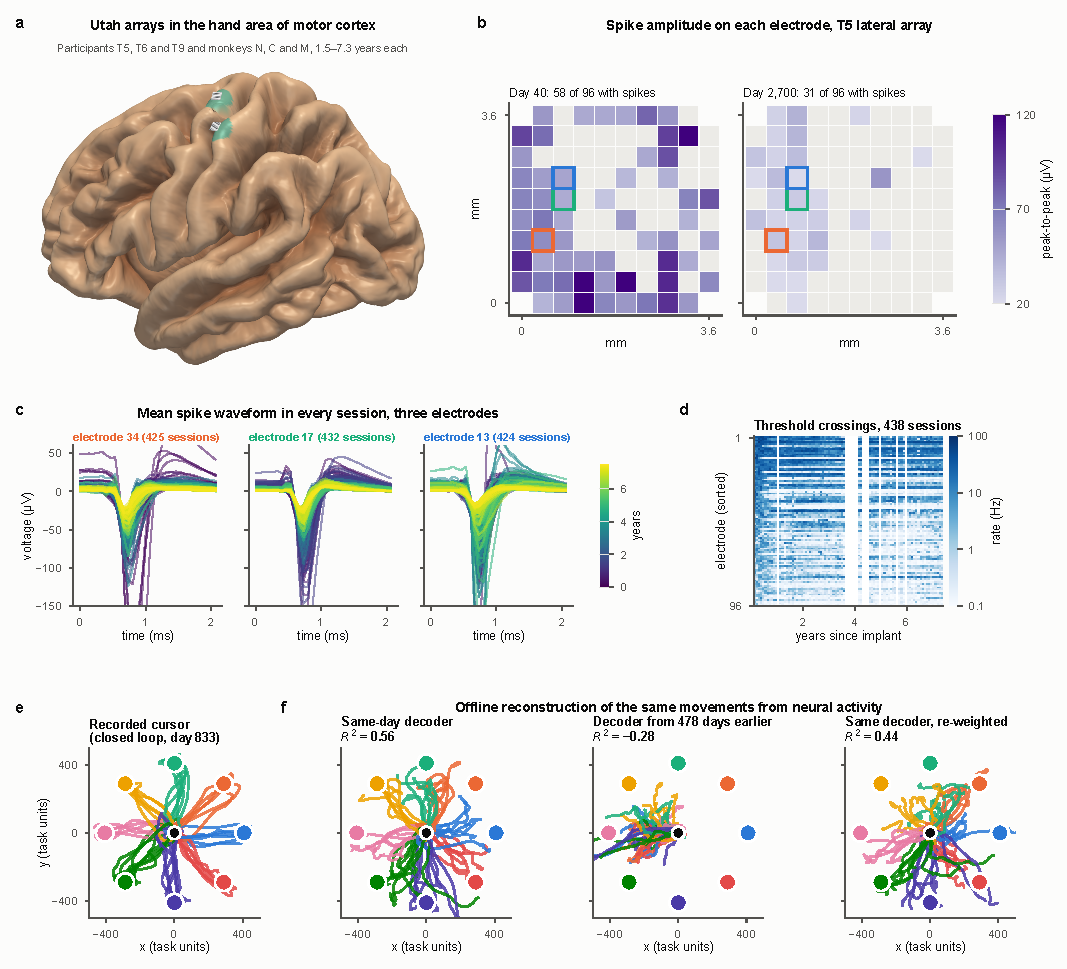
\includegraphics[width=170mm]{fig1_overview.pdf}}
\caption{\textbf{Data and analysis design.} \textbf{a}, Sessions used in this study, by individual and analysis,
against years since each individual's first session. Each tick is one session. Blue, decoder drift (monkeys N, C and M;
human participants T6, T5 and T9); green, electrode statistics (20 arrays in 14 BrainGate participants); orange,
closed-loop monitoring (T11 and T5). Counts are per analysis; some human sessions enter more than one analysis.
\textbf{b}, The correction ladder. A decoder trained on day $i$ is tested on a later day $j$ after increasingly powerful
corrections: none; label-free corrections (rescaling each channel, aligning neural activity); and corrections that use
labelled trials from day $j$ (re-learning one weight per channel; refitting the decoder while shrinking it toward the
old one). A decoder trained on day $j$ is the reference.}
\label{fig:overview}
\end{figure}

\subsection*{Decoders decay at rates that differ a hundredfold}

Without any correction, decoders failed: reusing the training day's normalization gave median $R^2$ below zero at most
gaps (Supplementary Table~2). We therefore treat the renormalized fixed decoder as the baseline.

How much accuracy survives a single night differed between species (Fig.~\ref{fig:decay}a,b). For true one-day gaps,
retention was \val{N:strict1} in monkey N (95\% confidence interval \val{N:strict1ci}; $n = \val{N:strict1n}$ pairs),
\val{C:strict1} in monkey C (\val{C:strict1ci}; $n = \val{C:strict1n}$) and \val{M:strict1} in monkey M
(\val{M:strict1ci}; $n = \val{M:strict1n}$). In participant T9 it was \val{T9:strict1} (\val{T9:strict1ci};
$n = \val{T9:strict1n}$). One-day pairs were rare in T6 ($n = \val{T6:strict1n}$; retention \val{T6:strict1}, interval
\val{T6:strict1ci}) and T5 ($n = \val{T5:strict1n}$). At two days, retention was \val{T6:strict2} in T6
($n = \val{T6:strict2n}$) and \val{T5:strict2} in T5 ($n = \val{T5:strict2n}$). Across the six individuals, retention
after one to two days differed (Kruskal--Wallis test, $H = \val{kw:H}$, d.f.~$= \val{kw:df}$, $P = \val{kw:P}$; one
value per training session).

Longer-term decay differed far more. Retention fell to one half within \val{T9:thalf} days in T9, \val{T5:thalf} days in
T5, \val{N:thalf} days in monkey N and \val{C:thalf} days in monkey C. It took \val{M:thalf} days in monkey M and
\val{T6:thalf} days in T6 (Fig.~\ref{fig:decay}a,c). The reference decoder itself stayed equally accurate across gaps
(Supplementary Table~2), so the decline reflects a growing mismatch between the decoder and the day, not poorer
recordings.

\begin{figure}[tbp]
\centering
\makebox[\textwidth][c]{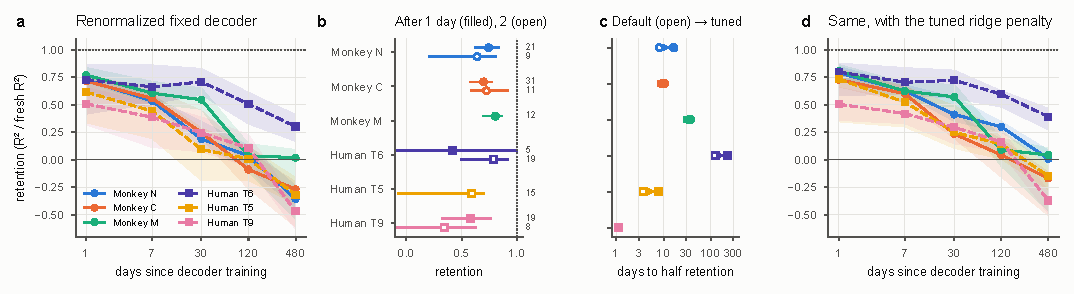
\includegraphics[width=170mm]{fig2_decay.pdf}}
\caption{\textbf{Decoders decay at rates that differ between individuals, and weak regularization exaggerates decay.}
\textbf{a}, Retention of the renormalized fixed decoder (decoding $R^2$ divided by that of a decoder trained on the test
day) against days since training, with the ridge penalty used in the original dataset papers. Lines show medians and
bands show 95\% confidence intervals from a cluster bootstrap over training sessions. Circles and solid lines, monkeys;
squares and dashed lines, humans. Blue, monkey N; orange, monkey C; green, monkey M; purple, T6; amber, T5; pink, T9.
\textbf{b}, Retention after exactly one day (filled) and two days (open), with 95\% confidence intervals; numbers give
pairs. Markers are omitted when fewer than three pairs were available. \textbf{c}, Days until retention falls to one
half with the default penalty (open) and with the tuned penalty (filled; logarithmic axis). \textbf{d}, As in
\textbf{a}, for decoders trained with the tuned penalty ($\alpha = 10^4$). Pair counts are given in Supplementary
Table~2.}
\label{fig:decay}
\end{figure}

\subsection*{Weak regularization exaggerates decay}

Part of the measured decay came from the decoder rather than the recordings. With a ridge penalty of $\alpha = 10^4$
instead of the small values used in the original dataset papers\cite{temmar2025}, the time to half retention rose from
\val{N:thalf} to \val{N:thalftuned} days in monkey N and from \val{T6:thalf} to \val{T6:thalftuned} days in T6
(Fig.~\ref{fig:decay}c,d). It changed little in monkeys C (\val{C:thalf} to \val{C:thalftuned} days) and M
(\val{M:thalf} to \val{M:thalftuned} days), whose original decoders were already more strongly regularized, and in T5
(\val{T5:thalf} to \val{T5:thalftuned} days) and T9 (\val{T9:thalf} to \val{T9:thalftuned} days). Per training session,
absolute $R^2$ on later days rose by a median of \val{N:tunedabsdiff} in monkey N (two-sided Wilcoxon signed-rank test,
$P = \val{N:tunedabsp}$) and \val{T6:tunedabsdiff} in T6 ($P = \val{T6:tunedabsp}$).

A simple rule captures this benefit using training-day data only: choose the largest penalty whose same-day accuracy
stays within 1\% of the best (Fig.~\ref{fig:recipes}a,b and Supplementary Table~6). Compared with $\alpha = 0.1$, it
raised cross-day $R^2$ in every individual, with session-level median gains of \val{N:rulemed} in monkey N
(\val{N:rulepos} of \val{N:rulen} sessions; $P = \val{N:rulep}$), \val{T6:rulemed} in T6 ($P = \val{T6:rulep}$),
\val{T5:rulemed} in T5 ($P = \val{T5:rulep}$) and \val{T9:rulemed} in T9 ($P = \val{T9:rulep}$). Gains were small in
monkeys C (\val{C:rulemed}) and M (\val{M:rulemed}). Same-day accuracy did not fall (median change \val{M:rulesame} to
$+$\val{T6:rulesame}). Ordinary same-day tuning chose similar penalties in most individuals (Methods), so the lesson is
that small default penalties exaggerate drift, rather than that cross-validation fails.

\subsection*{Re-weighting each channel restores most accuracy in people}

We next asked what kind of change the remaining loss reflects. Re-learning one weight per channel in front of the frozen
decoder lets each channel's contribution grow, shrink or vanish, but keeps the decoder's pattern across time lags and
outputs. In all three people, this correction restored most of the lost accuracy at every gap (Fig.~\ref{fig:reweight}a).
It recovered \val{T6:recmin}--\val{T6:recmax}\% of the loss in T6, \val{T5:recmin}--\val{T5:recmax}\% in T5 and
\val{T9:recmin}--\val{T9:recmax}\% in T9 (medians per gap; Fig.~\ref{fig:reweight}b). Retention after re-weighting stayed
between \val{T9:gainretmin} and \val{T6:gainretmax} even 480 days after training. In the monkeys, the same correction
recovered \val{N:recmin}--\val{N:recmax}\% of the loss in monkey N, \val{C:recmin}--\val{C:recmax}\% in C and
\val{M:recmin}--\val{M:recmax}\% in M, and retention after re-weighting fell to \val{C:gainret480}--\val{N:gainret480} at
480 days.

The human result did not depend on the decoder. A recurrent network decoder (Methods), regularized to avoid
memorizing the closed-loop sessions, was as accurate as the linear decoder in people (median $R^2$ \val{T6:nnown},
\val{T5:nnown} and \val{T9:nnown} versus \val{T6:linown}, \val{T5:linown} and \val{T9:linown}). Re-weighting its input
channels recovered \val{T6:nnrecmin}--\val{T6:nnrecmax}\%, \val{T5:nnrecmin}--\val{T5:nnrecmax}\% and
\val{T9:nnrecmin}--\val{T9:nnrecmax}\% of its loss (Fig.~\ref{fig:reweight}b). In monkeys the network was more accurate
than the linear decoder (median $R^2$ higher by \val{N:nnowndiff}, \val{C:nnowndiff} and \val{M:nnowndiff}), but
re-weighting again recovered less at long gaps (Supplementary Table~3).

Could the species difference reflect what was decoded? Human decoders predicted a two-dimensional direction, whereas
monkey decoders predicted four kinematic signals. We therefore rebuilt the reaching monkeys' sessions to decode the
direction of hand movement only, mirroring the human target (Methods). Re-weighting then recovered
\val{C:matchrec1}\% of the loss at one day and \val{C:matchrec480}\% at 480 days in monkey C, and \val{M:matchrec1}\% and
\val{M:matchrec480}\% in monkey M (Fig.~\ref{fig:reweight}c). The decoded variable therefore does not explain the
difference.

How much labelled data does re-weighting need in people? Pooled over the three participants and all gaps, retention
after re-weighting was \val{hum:effL3n20} with 20 labelled trials, \val{hum:effL3n50} with 50 and \val{hum:effL3n300} with
300, against \val{hum:effnone} without labels (Fig.~\ref{fig:reweight}d). A fresh decoder reached \val{hum:effL6n20}
with 20 trials and \val{hum:effL6n50} with 50. A trial lasted about 1.6--3.9~s in these sessions, so 20 trials take
under a minute in T5 and T6.

\begin{figure}[tbp]
\centering
\makebox[\textwidth][c]{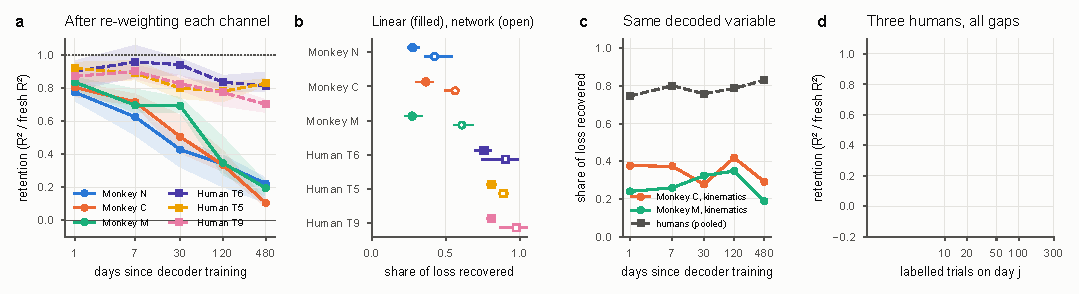
\includegraphics[width=170mm]{fig3_reweight.pdf}}
\caption{\textbf{Re-weighting each channel restores most accuracy in people.} \textbf{a}, Retention after re-learning
one weight per channel in front of the frozen linear decoder, with up to 300 labelled trials from the test day. Lines,
bands and colours as in Fig.~\ref{fig:decay}a. \textbf{b}, Share of the loss recovered by re-weighting, (re-weighted
$R^2$ minus renormalized $R^2$)/(reference $R^2$ minus renormalized $R^2$), for the linear decoder (filled) and a
recurrent network decoder (open), median over all pairs with 95\% cluster-bootstrap confidence intervals. \textbf{c},
Share of the loss recovered in the reaching monkeys when decoding hand kinematics (solid) or hand-movement direction
only (dotted), the variable decoded in the human sessions, with the human median for comparison (grey). \textbf{d},
Retention against the number of labelled trials on the test day, pooled over the three human participants and all
gaps, for re-weighting channels, refitting the decoder while shrinking it toward the old one, and training a fresh
decoder. The dotted line marks the renormalized fixed decoder, which uses no labels.}
\label{fig:reweight}
\end{figure}

\subsection*{Rescaling each channel is the label-free step that matters}

Several methods realign neural activity to a reference day without labels\cite{degenhart2020,gallego2020,ma2023,
karpowicz2025}. Their benefits were usually measured against a fixed decoder or against one whose channel means alone
were updated\cite{ma2023,wilson2025}. We compared four label-free corrections with renormalization, which rescales each
channel (Fig.~\ref{fig:labelfree}a and Supplementary Table~4).

Rotating the dominant neural subspace onto the training day by orthogonal Procrustes analysis\cite{schonemann1966} did
not help. Applied after updating channel means only, it lowered $R^2$ in monkey N by \val{N:rotmeandiff} (two-sided
Wilcoxon signed-rank test over training sessions, $P = \val{N:rotmeanp}$). Applied after renormalization, it lowered $R^2$
by \val{N:rotrendiff} ($P = \val{N:rotrenp}$); in the humans the changes were \val{T6:rotrendiff},
\val{T5:rotrendiff} and \val{T9:rotrendiff}. Renormalization itself improved on updating means only by
\val{N:renmeandiff} in monkey N ($P = \val{N:renmeanp}$). Matching the full covariance of the channels (CORAL\cite{sun2016})
changed $R^2$ by \val{N:coraldiff} in monkey N ($P = \val{N:coralp}$), \val{M:coraldiff} in M, and
\val{T6:coraldiff}, \val{T5:coraldiff} and \val{T9:coraldiff} in the humans. A faithful implementation of the
factor-analysis stabilizer of Degenhart and colleagues\cite{degenhart2020} improved on its own fixed latent decoder in
none of the monkeys (change \val{N:stabfixdiff} in N, \val{M:stabfixdiff} in M) and did not consistently beat
renormalization in the humans (changes \val{T6:stabrendiff}, \val{T5:stabrendiff} and \val{T9:stabrendiff}). That method
was designed for closed-loop use with a latent decoder, and offline tests may understate it. In these data, however,
the useful label-free step was to rescale each channel.

\subsection*{Neural change adds little beyond time since calibration}

A monitor that warns when a decoder is failing could make recalibration less frequent. MINDFUL scores instability as
the divergence between distributions of neural features, or of decoder outputs, on a test day and a reference
day\cite{pun2024}. Such scores correlate with decoder error, but both grow with time since calibration, so a
correlation alone does not show that a score adds information.

Offline in monkey N (537 session pairs), elapsed time alone correlated with decoder accuracy (Spearman
$|\rho| = \val{mon:days}$; Fig.~\ref{fig:labelfree}b). Neural divergence correlated more weakly
($|\rho| = \val{mon:neuralraw}$), and its partial correlation fell to \val{mon:neuralpart} after controlling for elapsed
time. Output divergence behaved the same way ($|\rho| = \val{mon:outraw}$, partial \val{mon:outpart}). Adding both
divergences to elapsed time slightly increased the cross-validated error of predicted $R^2$ (\val{mon:maeboth} versus
\val{mon:maedays}). A broader set of label-free statistics fared no better (Supplementary Note~1), although day-to-day
performance beyond the time trend was reliable (split-half reliability 0.84).

We then re-analysed the public MINDFUL data, in which T11 and T5 controlled a cursor in closed loop with a fixed decoder
(Fig.~\ref{fig:labelfree}c and Supplementary Table~5). In T11 (\val{T11:mf:days} days), neural divergence correlated
with angular error ($r = \val{T11:mf:nraw}$), consistent with the original report\cite{pun2024}. Most of this
association was shared with elapsed time (partial $r = \val{T11:mf:npart}$), and adding neural divergence did not
improve leave-one-day-out prediction of error (\val{T11:mf:dn}\textdegree{} versus \val{T11:mf:days}\textdegree{}).
Output divergence kept a partial correlation of \val{T11:mf:opart}, and adding it reduced the error to
\val{T11:mf:do}\textdegree. In T5, error was barely related to elapsed time over \val{T5:mf:days} days
($r = \val{T5:mf:rdays}$), and both divergences tracked error (partial $r = \val{T5:mf:npart}$ for neural and
\val{T5:mf:opart} for output divergence). These comparisons involve few days, and output divergence and angular error
are both computed from the cursor's motion, so part of their link is mechanical. Within these limits, elapsed time was
as good a guide as neural statistics in most comparisons.

\begin{figure}[tbp]
\centering
\makebox[\textwidth][c]{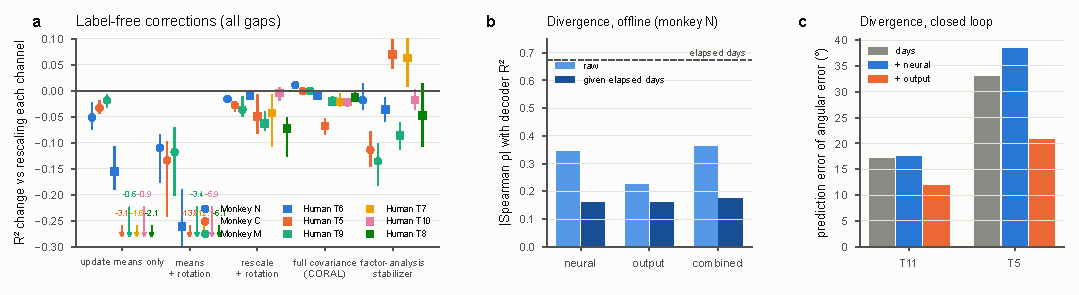
\includegraphics[width=170mm]{fig4_labelfree.pdf}}
\caption{\textbf{Label-free corrections and monitoring add little to rescaling and elapsed time.} \textbf{a}, Change in
decoding $R^2$ relative to renormalization (rescaling each channel) for five label-free corrections, per individual,
averaged over each training session's pairs at gaps up to 120 days. Points show medians over training sessions and
bars show 95\% cluster-bootstrap confidence intervals. Colours and markers as in Fig.~\ref{fig:decay}. \textbf{b},
Offline monitoring in monkey N (537 pairs): absolute Spearman correlation between decoder $R^2$ and the divergence of
neural features, decoder outputs or both, before (light) and after (dark) controlling for elapsed days. The dashed
line marks elapsed days alone. \textbf{c}, Closed-loop monitoring in the public MINDFUL data: leave-one-day-out mean
absolute error in predicting angular error from elapsed days (grey), with neural divergence added (blue) or with output
divergence added (orange).}
\label{fig:labelfree}
\end{figure}

\subsection*{Shrinking toward the old decoder makes small recalibrations safe}

When labelled data are scarce, refitting a decoder can make it worse. In monkey N (86 session pairs), we refitted the
decoder by ridge regression shrunk toward the old decoder, penalizing changes in both the weights and the
intercept\cite{kuzborskij2013,orsborn2012,dangi2013} (Fig.~\ref{fig:recipes}c and Supplementary Table~7). Choosing the
shrinkage strength by cross-validation on a few trials was unreliable: with 10 trials, \val{harm:10:cv}\% of
recalibrations ended worse than no recalibration (Fig.~\ref{fig:recipes}d). A fixed strong shrinkage, the value that
worked best on pairs from other training sessions, lowered this to \val{harm:10:hist}\% (exact McNemar test on paired
outcomes, $P = \val{mcn:10:p}$; Holm-adjusted over five data budgets, $P = \val{mcn:10:holm}$). With 20 trials the rates
were \val{harm:20:cv}\% and \val{harm:20:hist}\% ($P = \val{mcn:20:p}$; adjusted $P = \val{mcn:20:holm}$). With 50 or
more trials, and at gaps of 30 days or more, refitting from scratch did as well as the shrunk refit.

\begin{figure}[tbp]
\centering
\makebox[\textwidth][c]{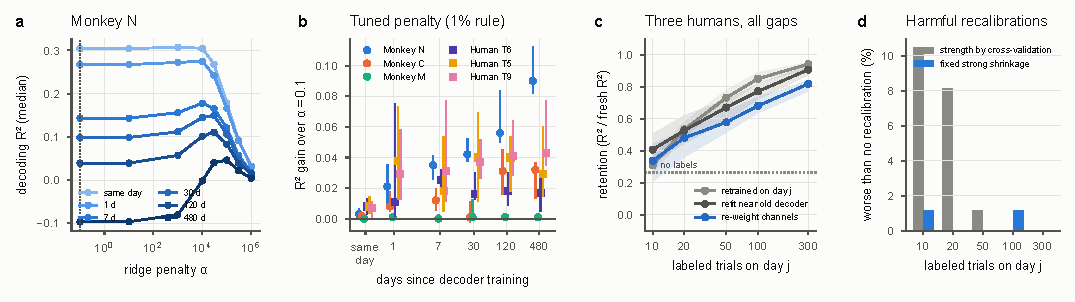
\includegraphics[width=170mm]{fig5_recipes.pdf}}
\caption{\textbf{Simple recipes for robust decoders.} \textbf{a}, Median decoding $R^2$ in monkey N against the ridge
penalty $\alpha$, on held-out trials of the training day (lightest) and on sessions 1, 7, 30, 120 and 480 days later
(darker). The dotted line marks $\alpha = 0.1$, the value used in the original dataset paper. \textbf{b}, Gain in $R^2$
from the 1\% rule (largest $\alpha$ whose same-day $R^2$ is within 1\% of the best) over $\alpha = 0.1$, on the same
day and at each gap, per individual; medians with 95\% cluster-bootstrap confidence intervals. \textbf{c}, Retention in
monkey N against the number of labelled trials on the test day, pooled over gaps, for refitting the decoder while
shrinking it toward the old one, training a fresh decoder and re-weighting channels. \textbf{d}, Percentage of
recalibrations (86 pairs) that ended more than 0.01 $R^2$ below the renormalized fixed decoder, with the shrinkage
strength chosen by cross-validation on the available trials (grey) or fixed at the value that worked best on other
training sessions (blue).}
\label{fig:recipes}
\end{figure}

\subsection*{Brief electrode silences are fluctuation, long ones are real}

We next asked how single electrodes change over years. We used the BrainGate yield data, which report threshold-crossing
rates and impedance for every electrode in every session\cite{hahn2026}, and the matching data from monkey N. An
electrode was active when its threshold-crossing rate exceeded 2~Hz, the definition used by BrainGate\cite{hahn2026}.
Array yield and impedance declined over years in both species (Fig.~\ref{fig:electrodes}a,b). Impedance fell in 17 of
18 human arrays with measurements (median Spearman $\rho$ with time $-0.92$) and in monkey N, from a median of
302~k$\Omega$ in the first year to 171~k$\Omega$ in the fourth ($\rho = -0.88$), replicating earlier
reports\cite{barrese2013,sponheim2021,chen2023,bjanes2025,hahn2026}.

Electrodes often fell silent and later recovered, but most such events were fluctuation rather than failure and repair
(Fig.~\ref{fig:electrodes}c and Supplementary Table~10). Of \val{rev:base:sil} initially active human electrodes that
stayed below threshold for at least three consecutive sessions, \val{rev:base:frac}\% later recovered for at least three
sessions. The same statistic computed after randomly shuffling each electrode's session order, which destroys any
temporal process, gave \val{rev:shuffle_null:frac}\%. The match held when the threshold was fixed in microvolts for
each electrode, so that changes in noise level could not move it (\val{rev:fixed_uv:frac}\% versus
\val{rev:shuffle_fixed_uv:frac}\%), and when silence required rates below 0.5~Hz (\val{rev:deep:frac}\% versus
\val{rev:shuffle_deep:frac}\%). Silences lasting at least 30 days were different. They were twice as common as in the
shuffled data (\val{rev:long_silence:sil} versus \val{rev:shuffle_long:sil}), and \val{rev:long_silence:frac}\% of them
ended in recovery, more than in the shuffled data (\val{rev:shuffle_long:frac}\%; Fisher's exact test,
$P = \val{rev:long:P}$). Recovery here means the electrode again recorded spiking, not necessarily from the same
neuron.

Spiking declined somewhat faster at the edge of the array than in its interior (Fig.~\ref{fig:electrodes}d). Among
initially active electrodes, the edge decline was steeper in \val{edge:raw:neg} of \val{edge:raw:n} human arrays with at
least 10 such electrodes (one-sided Wilcoxon signed-rank test with the array as the unit, $P = \val{edge:raw:wil}$), and
decline correlated with distance from the array centre ($P = \val{edge:dist:wil}$). After adjusting for each electrode's
initial firing rate, the edge effect weakened (\val{edge:adj:neg} of \val{edge:adj:n} arrays; $P = \val{edge:adj:wil}$).
In monkey N, edge electrodes declined faster within both arrays for threshold crossings but not for spike-band power.
These trends agree with models in which micromotion strains tissue most at the array edges\cite{forrest2025}, but they
are modest and partly explained by initial activity.

\begin{figure}[tbp]
\centering
\makebox[\textwidth][c]{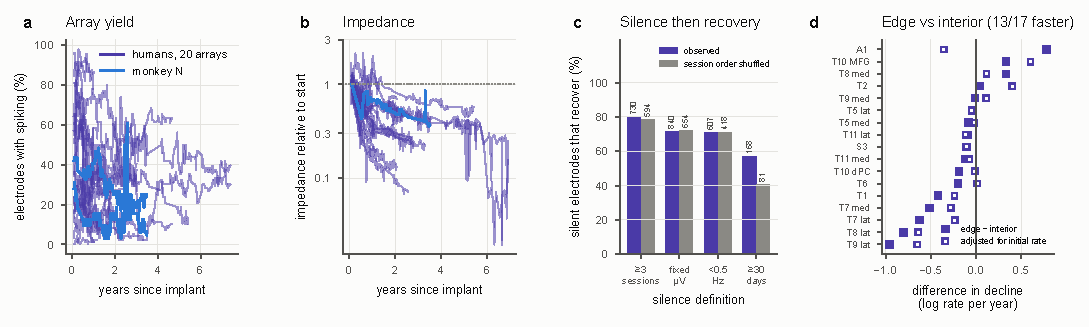
\includegraphics[width=170mm]{fig6_electrodes.pdf}}
\caption{\textbf{Brief electrode silences are fluctuation; long silences are real.} \textbf{a}, Percentage of
electrodes with spiking activity (threshold-crossing rate of at least 2~Hz) against years since implant, for 20 human
arrays (purple) and the two arrays of monkey N (blue). \textbf{b}, Median impedance of each array relative to its
first sessions (logarithmic axis). \textbf{c}, Percentage of silent episodes in initially active human electrodes
that ended in recovery (at least three sessions above 4~Hz), observed (purple) and after shuffling each electrode's
session order (grey), for four definitions of silence: at least three sessions below 2~Hz; the same with a fixed
microvolt threshold per electrode; below 0.5~Hz; and lasting at least 30 days. Numbers give silent episodes.
\textbf{d}, Difference in the decline of log threshold-crossing rate per year between edge and interior electrodes,
per human array with at least 10 initially active electrodes, unadjusted (filled) and adjusted for initial firing
rate (open). Negative values mean faster decline at the edge.}
\label{fig:electrodes}
\end{figure}

\subsection*{A calibrated simulator predicts untested corrections}

Methods for stable decoding are hard to compare without a common test bed\cite{karpowicz2024falcon}. We built a
feature-level simulator that takes a real session and returns it as it might appear days to years later (Methods). It
combines mixing of signals between channels, gradual turnover of each channel's tuning and switching of electrodes
between active and silent states. Switching rates came from monkey N's electrode statistics, and the mixing and turnover
parameters were calibrated so that the simulated correction ladder matched monkey N's during its first 700 days
(root-mean-square error \val{sim:rms} in retention; Fig.~\ref{fig:sim}a).

We tested the simulator on the later days, which it had not seen, against two baselines (Fig.~\ref{fig:sim}b). A
simulator without drift was far worse (median absolute error \val{sim:fit:nodrift}--\val{sim:budget:nodrift}). A
stronger baseline simply reused the median retention measured in the first 700 days. For the corrections used in
calibration, and for different amounts of labelled data, this empirical curve was as good as or better than the
simulator (\val{sim:fit:early} versus \val{sim:fit:sim}, and \val{sim:budget:early} versus \val{sim:budget:sim}).
For corrections that the simulator was not fitted to, it was clearly better (\val{sim:unfit:sim} versus
\val{sim:unfit:early}). The simulator is therefore most useful for predicting how new corrections will behave. Real
decoders decayed more slowly in the later years, and a calibration on that period gave weaker session-to-session
mixing (\val{sim:mix0late} versus \val{sim:mix0}) and slower turnover (time constant \val{sim:taurholate} versus
\val{sim:taurho} days), suggesting that drift slows as an implant ages in this monkey. Training decoders on simulated
futures helped little ($R^2$ higher by \val{aug:sim}) compared with stronger regularization (\val{aug:ridge_reg}) or
training on several past sessions (\val{aug:multi}; Supplementary Table~12).

\begin{figure}[tbp]
\centering
\makebox[\textwidth][c]{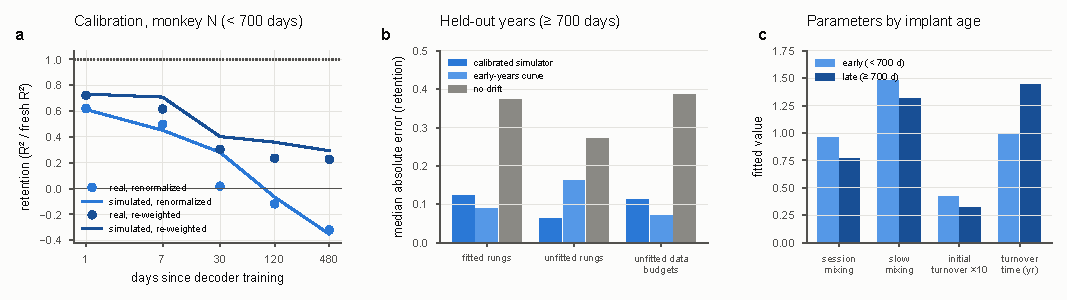
\includegraphics[width=170mm]{fig7_simulator.pdf}}
\caption{\textbf{A calibrated simulator predicts untested corrections.} \textbf{a}, Calibration on monkey N sessions
before day 700. Points show real median retention and lines show the calibrated simulator, for the renormalized fixed
decoder and after re-weighting channels. \textbf{b}, Validation on sessions after day 700: median absolute error
between predicted and real retention for corrections used in calibration, corrections not used in calibration and
amounts of labelled data not used in calibration. Dark blue, calibrated simulator; light blue, the median retention
measured before day 700; grey, the simulator with drift switched off. \textbf{c}, Parameters calibrated separately on
early ($<700$ days) and late ($\geq700$ days) sessions: session-to-session mixing, slow mixing, initial turnover
($\times10$) and turnover time constant (years).}
\label{fig:sim}
\end{figure}

\section*{Discussion}

We measured how decoders and electrodes change over years in three monkeys and 14 people with one pipeline. The
central finding is that in people, most of the accuracy a decoder loses over days to more than a year is recovered by
re-learning one weight per recording channel. This held in all three participants with decoding data, for linear and
recurrent decoders, and with little labelled data. In monkeys, the same correction recovered much less at long gaps,
even when we decoded the same variable.

This result has a simple interpretation. In these human recordings, the decoder's pattern across time lags and
outputs remained valid for each channel, while the strength with which each channel carried the decoded signal changed.
It agrees with the observation that tuning parameters on the same electrode tend to change together between
days\cite{bishop2014}. Our results do not reveal the cause. Changes in the number or proximity of neurons near each
electrode would act this way\cite{polikov2005,kozai2015}, as would changes in noise. Why monkeys differ is also open.
The human arrays were older at the start of recording, the human tasks were closed-loop, and the cortical areas and
species differ. Each of these could change how tuning evolves.

The practical implication is that recalibration in people can be small. Re-learning one weight per channel requires a
short block of labelled trials, adds few parameters and keeps the decoder that the user has learned to control. It
complements label-free methods, which in our data could not recover this kind of change beyond rescaling each channel.
Three further recipes follow from our results. Daily per-channel renormalization should be the baseline against which
new methods are compared. Ridge penalties should be tuned rather than left at small defaults, because weak
regularization exaggerates apparent drift. And when recalibrating from a few trials, shrinking toward the previous
decoder, including its intercept, avoids recalibrations that do more harm than good.

Decay rates varied about a hundredfold between individuals, from one day to several months to lose half of the accuracy.
A fixed recalibration schedule will therefore be wrong for many users. The monitoring analyses suggest that statistics
of neural change are a weak guide to when recalibration is needed, beyond elapsed time. Divergence of the decoder's
output was more informative in closed loop, although part of that link is mechanical. Monitoring studies should report
correlations after controlling for elapsed time and compare against a time-only baseline.

The electrode analyses refine common descriptions of array decline. Electrode activity near the yield threshold
fluctuated strongly from session to session, and most short silences were no more than that. Yield counts from single
sessions are therefore noisy, and decoders should not discard channels permanently after a few silent sessions.
Silences lasting over a month were real and still reversed in more than half of cases. The edge effect we found is
modest and partly explained by initial activity. Hahn and colleagues analysed yield, decoding signal quality and tuning
stability in the same human data\cite{hahn2026}. We add electrode-level analyses of silence and recovery with a
shuffled null, and a test of edge-biased spiking loss with the array as the unit.

Our study has limitations. All analyses were offline. In closed loop, users adapt to their decoder\cite{gilja2012},
which could slow or hide decay. Human decoding labels were inferred from the direction from cursor to target, and the
online decoder shaped both the neural activity and the cursor path. Three participants and three monkeys cannot
establish population rates, and the datasets differ in task, signal type, array placement and implant age. The simulator
is calibrated to feature-level statistics in one monkey and does not model biophysics. Finally, we tested label-free
methods offline, where they may perform differently than in closed loop.

Long-term public datasets made this study possible. We release our code, derived results and the calibrated simulator
so that others can test methods against realistic drift. Our results suggest that durable clinical decoders may need
less effort than often assumed: a brief re-weighting of channels may keep a familiar decoder working for months.

\section*{Methods}

\subsection*{Datasets and ethics}

All data were public and de-identified. The original studies obtained ethical approval and informed consent, as
described in the cited publications. We collected no new data.

\textit{Monkey N} (LINK; DANDI Archive 001201\cite{data_link}; ref.~\cite{temmar2025}). One rhesus macaque had Utah arrays
in the hand area of primary motor cortex\cite{nason2021}. The release contains 312 sessions on 303 days over 1,242 days,
in which the monkey moved two finger groups to targets in centre-out or random-target blocks. We used the 96 released
channels (64 on the medial array and 32 on the lateral array), with spike-band power and threshold crossings at $-4.5$
times the root-mean-square noise in 20~ms bins\cite{nason2020}. Outputs were the position and velocity of the two
finger groups. Electrode impedance was stored on 228 days.

\textit{Monkeys C and M} (DANDI Archive 000688\cite{data_perich}; refs.~\cite{gallego2020,perich2018}). Both monkeys had
Utah arrays in motor and premotor cortex and performed centre-out and random-target reaching. Monkey C had 68 sessions
from October 2013 to October 2016, and monkey M had 28 sessions from January 2014 to June 2015. We summed the spikes of
all sorted units on each electrode in 20~ms bins, giving 96 (C) or 192 (M) channels. Hand position and velocity were
interpolated to bin centres.

\textit{BrainGate participants} (Dryad\cite{data_braingate}; ref.~\cite{hahn2026}). The yield data contain one recording
from each of 2,289 research sessions in 14 participants with 20 arrays (A1, S1--S3, T1--T3 and T5--T11). For every
electrode, they list threshold-crossing rates at several thresholds (with the threshold in microvolts), impedance and
grid position. Nineteen arrays were in the hand area of motor cortex and one was in the middle frontal gyrus. The
decoding data contain closed-loop cursor sessions with spike-band power in 10~ms bins, cursor and target positions and
the periods of attempted movement. We used all sessions of T6 (124 sessions over 3.1 years, one array, 96 channels), T5
(92 sessions over 7.2 years, two arrays, 192 channels) and T9 (117 sessions over 2.0 years, two arrays, 192 channels).
Sessions contained a median of 367, 551 and 275 trials, with median movement periods of 1.6, 1.7 and 3.9~s.

\textit{MINDFUL} (Dryad\cite{data_mindful}; ref.~\cite{pun2024}). Closed-loop cursor blocks in which T11 (15 days) and T5
(6 days) used a fixed decoder, with neural features in 20~ms bins (spike-band power for T11 and threshold crossings for
T5), the decoder's velocity output and the angular error of the cursor.

\subsection*{Features, decoders and accuracy}

For monkey N and the human participants we used spike-band power (human 10~ms bins averaged in pairs). For monkeys C and
M we used per-electrode spike counts. Each channel was z-scored with the mean and standard deviation of the decoding
session's training segment, computed without labels (renormalization). The linear decoder was ridge
regression\cite{hoerl1970} on 8 causal lags (160~ms) of the z-scored features, with an unpenalized intercept. The default
penalty was $\alpha = 0.1$ for monkey N and the humans, as in ref.~\cite{temmar2025}, and $\alpha = 1$ for monkeys C and
M, whose spike-count features are sparser. Outputs were finger position and velocity for monkey N, hand position and
velocity for monkeys C and M, and for the humans the intended movement direction, defined as the unit vector from cursor
to target during attempted movement. Accuracy was the coefficient of determination $R^2$, averaged over outputs and
computed on held-out trials of the test session. In monkey N the first 300 of 375 trials trained the decoder, as in
ref.~\cite{temmar2025}; in the other datasets the first 80\% of trials did.

The recurrent decoder was a long short-term memory network\cite{hochreiter1997} with 64 hidden units, input dropout\cite{srivastava2014} of
0.5 and 20-bin input windows (400~ms). It was trained with AdamW\cite{loshchilov2019} (learning rate $10^{-3}$, weight decay 0.01) for up to
4,000 iterations of 256 samples, with early stopping on the last 20\% of training trials checked every 100 iterations.
Without these measures, a 256-unit network memorized the human training sessions (training $R^2$ 0.97, test $R^2$
$-1.1$ on one session). The network ladder used 25 training sessions per individual chosen at random with a fixed seed.

\subsection*{Session pairs}

For each training session $i$ and target gap $g \in \{1, 7, 30, 120, 480\}$ days, we selected the later session $j$ of
the same task type whose gap was closest to $g$, within 25\% of $g$ or one day, whichever was larger. The one-day set
therefore contains one- and two-day gaps, which we report separately. In monkey N, 80 training sessions were drawn at
random with a fixed seed; the full monkey N set (537 pairs) also includes further gaps and was used for monitoring. All
human sessions were treated as one task type. Pair counts are listed in Supplementary Table~2.

\subsection*{Correction ladder}

Let $\mathbf{x}_j(t) \in \mathbb{R}^C$ be the raw features of test day $j$, $\boldsymbol{\mu}_d$ and
$\boldsymbol{\sigma}_d$ the channel means and standard deviations of day $d$, and $f_i$ the decoder trained on day $i$.

\begin{itemize}
\item \textit{No correction}: $f_i\big((\mathbf{x}_j - \boldsymbol{\mu}_i)/\boldsymbol{\sigma}_i\big)$.
\item \textit{Mean updating}: $f_i\big((\mathbf{x}_j - \boldsymbol{\mu}_j)/\boldsymbol{\sigma}_i\big)$.
\item \textit{Renormalization}: $f_i(\mathbf{z}_j)$ with $\mathbf{z}_j = (\mathbf{x}_j - \boldsymbol{\mu}_j)/
\boldsymbol{\sigma}_j$.
\item \textit{Re-weighting}: $f_i$ applied to $g_c z_{j,c}$ for each channel $c$, with one offset per output. The weights
$g_c$ were shrunk toward 1 and the offsets toward the old intercept; the penalty was chosen from
$\{10^{-6}, \ldots, 10^2\}$ by five-fold cross-validation over contiguous blocks of trials.
\item \textit{Ridge to prior}: a new decoder $(\mathbf{W}, \mathbf{b})$ fitted on the lagged features $\mathbf{H}$ of day
$j$ by minimizing
\begin{equation}
\|\mathbf{Y} - \mathbf{H}\mathbf{W} - \mathbf{1}\mathbf{b}^\top\|_F^2 + \lambda\left(\|\mathbf{W} - \mathbf{W}_i\|_F^2
+ \|\mathbf{b} - \mathbf{b}_i\|_2^2\right),
\label{eq:prior}
\end{equation}
where $(\mathbf{W}_i, \mathbf{b}_i)$ is the old decoder and $\lambda$ was chosen from $\{0.1, 1, \ldots, 10^6\}$ by
cross-validation.
\item \textit{Reference}: a decoder trained on day $j$'s training trials.
\end{itemize}

\noindent Supervised rungs used the first $n$ labelled trials of day $j$ ($n = 300$, or all training trials if fewer,
unless stated). Retention was the ratio of a rung's $R^2$ to the reference $R^2$ on the same test trials, and the share
of the loss recovered by re-weighting was $(R^2_{\text{reweight}} - R^2_{\text{renorm}})/(R^2_{\text{ref}} -
R^2_{\text{renorm}})$. The time to half retention was found by interpolating median retention linearly in log days. For
the network decoder, re-weighting was a learned per-channel gain and offset in front of the frozen network, and the
refit was fine-tuning with an $L_2$ penalty toward the old weights; penalties were chosen on the last 20\% of labelled
trials. We also computed a full input remap fitted by L-BFGS\cite{liu1989}; because it can represent any linear decoder
of the same form, we used it only as a calibration target for the simulator.

\textit{Matched-output control.} For monkeys C and M, sessions were rebuilt with a two-dimensional unit-vector target,
the direction of hand velocity, on bins where hand speed exceeded the session's 25th percentile. The ladder was run on
the same pairs.

\textit{Data efficiency in humans.} For 30 training sessions per participant (fixed seed), the ladder was run with
$n \in \{10, 20, 50, 100, 300\}$ labelled trials.

\subsection*{Label-free corrections}

\textit{Procrustes rotation.} Let $\mathbf{V}_i, \mathbf{V}_j \in \mathbb{R}^{C\times k}$ hold the top $k = 16$ principal
axes of the corrected training features on each day. The orthogonal matrix $\mathbf{R}$ minimizing
$\|\mathbf{V}_j\mathbf{R} - \mathbf{V}_i\|_F$ was found by Procrustes analysis\cite{schonemann1966}, and inputs were mapped
as $(\mathbf{I} - \mathbf{V}_j\mathbf{V}_j^\top)\mathbf{z} + \mathbf{V}_i\mathbf{R}^\top\mathbf{V}_j^\top\mathbf{z}$. We
applied it to renormalized features and, separately, to mean-updated features with $\mathbf{V}_j$ estimated from those
features.

\textit{CORAL.} Renormalized day-$j$ features were re-coloured to match day $i$'s covariance,
$\mathbf{z}' = \mathbf{C}_i^{1/2}\mathbf{C}_j^{-1/2}\mathbf{z}$\cite{sun2016}, with covariances shrunk 5\% toward a scaled
identity.

\textit{Factor-analysis stabilizer.} Following ref.~\cite{degenhart2020}, a factor-analysis model with 10 latent factors
was fitted to each day's renormalized training features, and a ridge decoder on 8 lags of the day-$i$ posterior latent
means was trained. On day $j$, a model fitted without labels was aligned to day $i$ by orthogonal Procrustes analysis of
the loadings of stable channels, found by iteratively keeping the 60\% of channels with the smallest loading residuals;
latents were then inferred from stable channels only and passed to the frozen latent decoder. The comparison baseline
reused the day-$i$ factor model on day $j$.

\subsection*{Monitoring analyses}

In monkey N, for every pair we computed Gaussian Kullback--Leibler divergences between days $i$ and $j$ of the
projections of renormalized features on day $i$'s top ten principal axes (neural divergence) and of the decoder's
outputs (output divergence). We report raw Spearman correlations with $R^2$, partial correlations given log elapsed days
and time-blocked cross-validated linear prediction of $R^2$. The additional statistics are described in Supplementary
Note~1. Split-half reliability of the residual after the time trend used alternating pairs of trials and the
Spearman--Brown formula. For the MINDFUL data we followed the original definitions\cite{pun2024}: non-overlapping 60~s
windows, divergences against the first day, and the median angular error over non-excluded trials (windows with fewer
than 500 valid bins skipped). We report Pearson and partial correlations given elapsed days, and leave-one-day-out
linear prediction of angular error; the reference day was excluded from evaluation.

\subsection*{Regularization and recalibration}

Ridge decoders were trained with $\alpha \in \{0.1, 10, 10^3, 10^4, 3\times10^4, 10^5, 3\times10^5, 10^6\}$ on 40
training sessions per individual (22 for monkey M) and evaluated on held-out same-day trials and on later sessions at
the five gaps. The 1\% rule chose the largest $\alpha$ whose median same-day $R^2$ was at least 99\% of the best median.
We compared it with each training session's own best same-day penalty: they did not differ in monkeys C and M or in
T6, and the rule added \val{N:rulevsbest} in monkey N ($P = \val{N:rulevsbestp}$). The tuned-penalty ladder repeated the
correction ladder on the same pairs with $\alpha = 10^4$ for both the day-$i$ and the reference decoders. For
recalibration with few trials we used 86 monkey N pairs and $n \in \{10, 20, 50, 100, 300\}$. The shrinkage $\lambda$ in
equation~(\ref{eq:prior}) was chosen per pair by cross-validation on the $n$ trials, or as the value with the best median
$R^2$ over pairs from other training sessions, which was $10^4$ for every pair with up to 50 trials. A recalibration was
harmful when its $R^2$ was more than 0.01 below that of the renormalized fixed decoder.

\subsection*{Electrode statistics}

Statistics were computed per array. An electrode was active in a session when its threshold-crossing rate at $-4.5$ times
the root-mean-square noise was at least 2~Hz. An initially active electrode (mean rate of at least 2~Hz over the first
three sessions) was silent when it stayed below threshold for at least three consecutive observed sessions, and
recovered when it later exceeded 4~Hz for at least three consecutive sessions. Missing sessions were skipped, not
imputed. Control analyses (Supplementary Table~10) used thresholds of $-3.5$ and $-5.5$ times the noise; a fixed
threshold per electrode in microvolts (its $-4.5$ value over the first three sessions, implemented by choosing in each
session the noise multiple whose microvolt threshold was closest); removal of sessions with array-wide shifts (absolute
median change in log rate above 1); a requirement for a mean waveform trough of at least 30~$\mu$V; silence below
0.5~Hz; and silences lasting at least 30 days. The null distribution randomly permuted each electrode's session order.
Switching rates were fitted by maximum likelihood to a two-state continuous-time Markov chain. For impedance, values of
4,000~k$\Omega$ or more were excluded and the trend was the Spearman correlation of the array median with day. For the
edge effect, edge electrodes were those on the outer ring of the grid ($10\times10$ in humans and $8\times8$ in monkey N),
each initially active electrode's decline was the slope of $\log(\text{rate} + 0.1)$ against years, and arrays with at
least 10 initially active electrodes were tested with the array as the unit. The adjusted analysis regressed slopes on
edge membership and initial log rate within each array.

\subsection*{Simulator}

The simulator transforms the z-scored features $\mathbf{Z} \in \mathbb{R}^{T\times C}$ of a real base session into those
of a simulated session $\Delta t$ days later (Supplementary Note~2). \textit{Mixing}: $\mathbf{Z} \leftarrow
\mathbf{Z}(\mathbf{I} + \mathbf{E})^\top$, with $\mathbf{E} = s(\Delta t)[(1 - \beta)\mathbf{G} + \beta\mathbf{L}]$, where
$\mathbf{G}$ is a Gaussian matrix with zero diagonal, $\mathbf{L}$ a Gaussian matrix restricted to grid neighbours,
$\beta = 0.5$ and $s(\Delta t)^2 = s_0^2 + [s_\infty(1 - e^{-\Delta t/\tau_s})]^2$. \textit{Turnover}: each channel
replaces a fraction $\rho_c$ of its signal by a unit with rotated tuning in the session's 20-dimensional latent space;
$\rho_c$ follows a beta distribution with mean $\rho_0 + (\rho_\infty - \rho_0)(1 - e^{-\Delta t/\tau_\rho})$ and
concentration 5. \textit{Silencing}: each channel active in the base session becomes silent with probability
$h_{\text{off}}/(h_{\text{off}} + h_{\text{on}})\,[1 - e^{-(h_{\text{off}} + h_{\text{on}})\Delta t}]$ and keeps 37\% of
its signal variance, the ratio of tuning strength of silent to active channels in monkey N. The switching rates
($h_{\text{off}} = \val{sim:hoff}$ and $h_{\text{on}} = \val{sim:hon}$ per day) were measured from monkey N's activity
in the calibration period. The six mixing and turnover parameters were calibrated on 12 base sessions before day 700 by
minimizing the summed squared difference between simulated and real median retention for three rungs at five gaps,
with the same correction code and regularization as for real data, using a 24-point Sobol search\cite{sobol1967}
followed by Nelder--Mead\cite{nelder1965}. Validation used 10 base sessions after day 700 and compared predicted and real
medians for all rungs and for $n \in \{20, 50, 100\}$. Augmentation added eight simulated futures per training session
($\Delta t$ log-uniform between 1 and 120 days) and was compared with stronger regularization, random channel dropout
with gain noise\cite{sussillo2016} and training on the three previous sessions.

\subsection*{Statistics}

Session pairs that share a training session are not independent. Confidence intervals for medians therefore came from a
cluster bootstrap over training sessions\cite{field2007} (2,000 resamples, percentile intervals), and paired tests used
one value per training session (two-sided Wilcoxon signed-rank tests, over gaps up to 120 days for label-free
corrections and over all gaps otherwise). Overnight retention was compared across individuals with a Kruskal--Wallis
test. Harmful recalibrations were compared with exact McNemar tests on paired outcomes, Holm-adjusted over the five data
budgets\cite{holm1979}. Revival rates were compared with Fisher's exact test. Electrode-edge tests used one value per
array (one-sided sign and Wilcoxon signed-rank tests; the direction was pre-specified from earlier work\cite{forrest2025}).
Exact $P$ values are reported. Analyses used Python 3.11 with NumPy, SciPy, pandas, scikit-learn and PyTorch.

\subsection*{Use of AI tools}

An AI assistant (Claude, Anthropic) was used to write analysis code, run analyses and draft the text under the
authors' direction. The authors reviewed the code, analyses and text and take full responsibility for the content.

\section*{Data availability}

All data analysed in this study are public. LINK (monkey N) is available from the DANDI Archive at
\url{https://doi.org/10.48324/dandi.001201/0.251023.2336}. The recordings of monkeys C and M are available at
\url{https://doi.org/10.48324/dandi.000688/0.250122.1735}. The BrainGate yield and decoding data are available from Dryad
at \url{https://doi.org/10.5061/dryad.x0k6djj1h}. The MINDFUL data are available from Dryad at
\url{https://doi.org/10.5061/dryad.n2z34tn5s}. All derived results underlying the figures and tables are provided in the
code repository.

\section*{Code availability}

All code, including the simulator with its calibrated parameters, is available at
\url{https://github.com/Imtiaj-Sajin/invasive-bci} under the MIT license. A versioned archive will be deposited on Zenodo
upon publication.

\backmatter

\bmhead{Acknowledgements}
We thank the participants of the BrainGate clinical trials and the teams who recorded and released the LINK, DANDI
000688, BrainGate and MINDFUL datasets. This work received no specific funding.

\bmhead{Author contributions}
All authors contributed to the study design, analysis, interpretation and writing, and approved the final manuscript.

\bmhead{Competing interests}
The authors declare no competing interests.

\begin{thebibliography}{99}

\bibitem{hochberg2006} Hochberg, L. R. et al. Neuronal ensemble control of prosthetic devices by a human with tetraplegia. \textit{Nature} \textbf{442}, 164--171 (2006).

\bibitem{hochberg2012} Hochberg, L. R. et al. Reach and grasp by people with tetraplegia using a neurally controlled robotic arm. \textit{Nature} \textbf{485}, 372--375 (2012).

\bibitem{collinger2013} Collinger, J. L. et al. High-performance neuroprosthetic control by an individual with tetraplegia. \textit{Lancet} \textbf{381}, 557--564 (2013).

\bibitem{pandarinath2017} Pandarinath, C. et al. High performance communication by people with paralysis using an intracortical brain--computer interface. \textit{eLife} \textbf{6}, e18554 (2017).

\bibitem{willett2021} Willett, F. R., Avansino, D. T., Hochberg, L. R., Henderson, J. M. \& Shenoy, K. V. High-performance brain-to-text communication via handwriting. \textit{Nature} \textbf{593}, 249--254 (2021).

\bibitem{willett2023} Willett, F. R. et al. A high-performance speech neuroprosthesis. \textit{Nature} \textbf{620}, 1031--1036 (2023).

\bibitem{card2024} Card, N. S. et al. An accurate and rapidly calibrating speech neuroprosthesis. \textit{N. Engl. J. Med.} \textbf{391}, 609--618 (2024).

\bibitem{wairagkar2025} Wairagkar, M. et al. An instantaneous voice-synthesis neuroprosthesis. \textit{Nature} \textbf{644}, 145--152 (2025).

\bibitem{card2026} Card, N. S. et al. Long-term independent use of an intracortical brain--computer interface for speech and cursor control. \textit{Nat. Med.} \textbf{32}, 2504--2510 (2026).

\bibitem{perge2013} Perge, J. A. et al. Intra-day signal instabilities affect decoding performance in an intracortical neural interface system. \textit{J. Neural Eng.} \textbf{10}, 036004 (2013).

\bibitem{chestek2011} Chestek, C. A. et al. Long-term stability of neural prosthetic control signals from silicon cortical arrays in rhesus macaque motor cortex. \textit{J. Neural Eng.} \textbf{8}, 045005 (2011).

\bibitem{downey2018} Downey, J. E., Schwed, N., Chase, S. M., Schwartz, A. B. \& Collinger, J. L. Intracortical recording stability in human brain--computer interface users. \textit{J. Neural Eng.} \textbf{15}, 046016 (2018).

\bibitem{bishop2014} Bishop, W. E. et al. Self-recalibrating classifiers for intracortical brain--computer interfaces. \textit{J. Neural Eng.} \textbf{11}, 026001 (2014).

\bibitem{barrese2013} Barrese, J. C. et al. Failure mode analysis of silicon-based intracortical microelectrode arrays in non-human primates. \textit{J. Neural Eng.} \textbf{10}, 066014 (2013).

\bibitem{sponheim2021} Sponheim, C. et al. Longevity and reliability of chronic unit recordings using the Utah, intracortical multi-electrode arrays. \textit{J. Neural Eng.} \textbf{18}, 066044 (2021).

\bibitem{bjanes2025} Bj{\aa}nes, D. A. et al. Quantifying physical degradation alongside recording and stimulation performance of 980 intracortical microelectrodes chronically implanted in three humans for 956--2130 days. \textit{Acta Biomater.} \textbf{198}, 188--206 (2025).

\bibitem{hahn2026} Hahn, N. V. et al. Performance of intracortical microelectrode arrays in people with implanted brain--computer interfaces over a 20-year period. \textit{Nat. Med.} (in the press); preprint at \url{https://doi.org/10.1101/2025.07.02.25330310} (2025).

\bibitem{jarosiewicz2015} Jarosiewicz, B. et al. Virtual typing by people with tetraplegia using a self-calibrating intracortical brain--computer interface. \textit{Sci. Transl. Med.} \textbf{7}, 313ra179 (2015).

\bibitem{sussillo2016} Sussillo, D., Stavisky, S. D., Kao, J. C., Ryu, S. I. \& Shenoy, K. V. Making brain--machine interfaces robust to future neural variability. \textit{Nat. Commun.} \textbf{7}, 13749 (2016).

\bibitem{orsborn2012} Orsborn, A. L., Dangi, S., Moorman, H. G. \& Carmena, J. M. Closed-loop decoder adaptation on intermediate time-scales facilitates rapid BMI performance improvements independent of decoder initialization conditions. \textit{IEEE Trans. Neural Syst. Rehabil. Eng.} \textbf{20}, 468--477 (2012).

\bibitem{dangi2013} Dangi, S., Orsborn, A. L., Moorman, H. G. \& Carmena, J. M. Design and analysis of closed-loop decoder adaptation algorithms for brain--machine interfaces. \textit{Neural Comput.} \textbf{25}, 1693--1731 (2013).

\bibitem{degenhart2020} Degenhart, A. D. et al. Stabilization of a brain--computer interface via the alignment of low-dimensional spaces of neural activity. \textit{Nat. Biomed. Eng.} \textbf{4}, 672--685 (2020).

\bibitem{gallego2020} Gallego, J. {\'A}., Perich, M. G., Chowdhury, R. H., Solla, S. A. \& Miller, L. E. Long-term stability of cortical population dynamics underlying consistent behavior. \textit{Nat. Neurosci.} \textbf{23}, 260--270 (2020).

\bibitem{ma2023} Ma, X. et al. Using adversarial networks to extend brain computer interface decoding accuracy over time. \textit{eLife} \textbf{12}, e84296 (2023).

\bibitem{karpowicz2025} Karpowicz, B. M. et al. Stabilizing brain--computer interfaces through alignment of latent dynamics. \textit{Nat. Commun.} \textbf{16}, 4662 (2025).

\bibitem{wilson2025} Wilson, G. H. et al. Long-term unsupervised recalibration of cursor-based intracortical brain--computer interfaces using a hidden Markov model. \textit{Nat. Biomed. Eng.} \textbf{10}, 1466--1484 (2025).

\bibitem{pun2024} Pun, T. K. et al. Measuring instability in chronic human intracortical neural recordings towards stable, long-term brain--computer interfaces. \textit{Commun. Biol.} \textbf{7}, 1363 (2024).

\bibitem{karpowicz2024falcon} Karpowicz, B. M. et al. Few-shot algorithms for consistent neural decoding (FALCON) benchmark. \textit{Adv. Neural Inf. Process. Syst.} \textbf{37} (2024).

\bibitem{chen2023} Chen, X. et al. Chronic stability of a neuroprosthesis comprising multiple adjacent Utah arrays in monkeys. \textit{J. Neural Eng.} \textbf{20}, 036039 (2023).

\bibitem{temmar2025} Temmar, H. et al. Long-term Intracortical Neural activity and Kinematics (LINK): an intracortical neural dataset for chronic brain--machine interfaces, neuroscience, and machine learning. \textit{Adv. Neural Inf. Process. Syst.} \textbf{38}, 154225--154247 (2025).

\bibitem{perich2018} Perich, M. G., Gallego, J. {\'A}. \& Miller, L. E. A neural population mechanism for rapid learning. \textit{Neuron} \textbf{100}, 964--976.e7 (2018).

\bibitem{nason2021} Nason, S. R. et al. Real-time linear prediction of simultaneous and independent movements of two finger groups using an intracortical brain--machine interface. \textit{Neuron} \textbf{109}, 3164--3177.e8 (2021).

\bibitem{hochreiter1997} Hochreiter, S. \& Schmidhuber, J. Long short-term memory. \textit{Neural Comput.} \textbf{9}, 1735--1780 (1997).

\bibitem{schonemann1966} Sch{\"o}nemann, P. H. A generalized solution of the orthogonal Procrustes problem. \textit{Psychometrika} \textbf{31}, 1--10 (1966).

\bibitem{sugiyama2007} Sugiyama, M., Krauledat, M. \& M{\"u}ller, K.-R. Covariate shift adaptation by importance weighted cross validation. \textit{J. Mach. Learn. Res.} \textbf{8}, 985--1005 (2007).

\bibitem{patil2024} Patil, P., Du, J.-H. \& Tibshirani, R. J. Optimal ridge regularization for out-of-distribution prediction. In \textit{Proc. 41st International Conference on Machine Learning} (PMLR, 2024).

\bibitem{kuzborskij2013} Kuzborskij, I. \& Orabona, F. Stability and hypothesis transfer learning. In \textit{Proc. 30th International Conference on Machine Learning} 942--950 (PMLR, 2013).

\bibitem{forrest2025} Forrest, A. M. et al. Finite element model predicts micromotion-induced strain profiles that correlate with the functional performance of Utah arrays in humans and non-human primates. \textit{J. Neural Eng.} \textbf{22}, 066008 (2025).

\bibitem{patel2023} Patel, P. R. et al. Utah array characterization and histological analysis of a multi-year implant in non-human primate motor and sensory cortices. \textit{J. Neural Eng.} \textbf{20}, 014001 (2023).

\bibitem{polikov2005} Polikov, V. S., Tresco, P. A. \& Reichert, W. M. Response of brain tissue to chronically implanted neural electrodes. \textit{J. Neurosci. Methods} \textbf{148}, 1--18 (2005).

\bibitem{kozai2015} Kozai, T. D. Y., Jaquins-Gerstl, A., Vazquez, A. L., Michael, A. C. \& Cui, X. T. Brain tissue responses to neural implants impact signal sensitivity and intervention strategies. \textit{ACS Chem. Neurosci.} \textbf{6}, 48--67 (2015).

\bibitem{gilja2012} Gilja, V. et al. A high-performance neural prosthesis enabled by control algorithm design. \textit{Nat. Neurosci.} \textbf{15}, 1752--1757 (2012).

\bibitem{data_link} Temmar, H. et al. LINK: Long-Term Intracortical Neural Activity and Kinematics. \textit{DANDI Archive} \url{https://doi.org/10.48324/dandi.001201/0.251023.2336} (2025).

\bibitem{nason2020} Nason, S. R. et al. A low-power band of neuronal spiking activity dominated by local single units improves the performance of brain--machine interfaces. \textit{Nat. Biomed. Eng.} \textbf{4}, 973--983 (2020).

\bibitem{data_perich} Perich, M. G., Miller, L. E., Azabou, M. \& Dyer, E. L. Long-term recordings of motor and premotor cortical spiking activity during reaching in monkeys. \textit{DANDI Archive} \url{https://doi.org/10.48324/dandi.000688/0.250122.1735} (2025).

\bibitem{data_braingate} Hahn, N. V. et al. Data from: Performance of intracortical microelectrode arrays in people with implanted brain--computer interfaces over a 20-year period. \textit{Dryad} \url{https://doi.org/10.5061/dryad.x0k6djj1h} (2026).

\bibitem{data_mindful} Pun, T. K. et al. Data from: Measuring instability in chronic human intracortical neural recordings towards stable, long-term brain--computer interfaces. \textit{Dryad} \url{https://doi.org/10.5061/dryad.n2z34tn5s} (2024).

\bibitem{hoerl1970} Hoerl, A. E. \& Kennard, R. W. Ridge regression: biased estimation for nonorthogonal problems. \textit{Technometrics} \textbf{12}, 55--67 (1970).

\bibitem{kingma2015} Kingma, D. P. \& Ba, J. Adam: a method for stochastic optimization. In \textit{Proc. 3rd International Conference on Learning Representations} (2015).

\bibitem{liu1989} Liu, D. C. \& Nocedal, J. On the limited memory BFGS method for large scale optimization. \textit{Math. Program.} \textbf{45}, 503--528 (1989).

\bibitem{fisher1925} Fisher, R. A. \textit{Statistical Methods for Research Workers} (Oliver and Boyd, 1925).

\bibitem{sobol1967} Sobol', I. M. On the distribution of points in a cube and the approximate evaluation of integrals. \textit{USSR Comput. Math. Math. Phys.} \textbf{7}, 86--112 (1967).

\bibitem{nelder1965} Nelder, J. A. \& Mead, R. A simplex method for function minimization. \textit{Comput. J.} \textbf{7}, 308--313 (1965).

\bibitem{field2007} Field, C. A. \& Welsh, A. H. Bootstrapping clustered data. \textit{J. R. Stat. Soc. B} \textbf{69}, 369--390 (2007).

\end{thebibliography}


\end{document}
